\documentclass{beamer}

\usepackage[T1]{fontenc}
\usepackage{lmodern} % provides bold-italic shapes

% Theme choice
\usetheme{Madrid}


\usepackage{amsmath}


\title{Kinetic Theory: Elements}
\author[Prof. Panesi]{Professor Marco Panesi\\[2cm]
\emph{Department of Mechanical and Aerospace Engineering}\\
University of California, Irvine}
\date{\today}

\begin{document}

% Slide 1: Title Slide
\begin{frame}
    \titlepage
\end{frame}

\begin{frame}
\frametitle{Kinetic Theory: Overview}
\begin{itemize}
    \item Focus on individual particles—molecules, atoms, and electrons.
    \item Collisions between particles in gases are key to kinetic theory.
    \item Energy transfer between translational, rotational, vibrational, and electronic modes requires {\bf via collisions}.
    \item In equilibrium, particle velocities follow {\bf Maxwell-Boltzmann} distribution.
    \item Frequency of collisions and mean free path are important characteristics.
\end{itemize}
\end{frame}

\begin{frame}
\frametitle{Importance of Particle Collisions}
\begin{itemize}
    \item In equilibrium, the system can reach thermodynamic and chemical equilibrium via collisions.
    \item In nonequilibrium, such as in rocket engines or hypersonic vehicles, particle collisions may not have enough time to occur.
    \item This leads to nonequilibrium behavior, requiring a deeper understanding of particle collision frequency.
    \item Transport properties such as viscosity, thermal conductivity, and diffusion depend on mean free path (distance between collisions).
\end{itemize}
\end{frame}

\begin{frame}
\frametitle{Introduction to Kinetic Theory}
\begin{itemize}
    \item Kinetic theory describes the microscopic motion of individual particles in a gas.
    \item Focus on translational motion in this chapter.
    \item Unlike classical thermodynamics, which deals with continuous systems, kinetic theory studies individual particle interactions.
    \item Understanding kinetic theory is essential for analyzing high-temperature chemically reacting gases and nonequilibrium flows.
\end{itemize}
\end{frame}

\begin{frame}
\frametitle{Application to High-Temperature Flows}
\begin{itemize}
    \item This section serves as a foundation for understanding high-temperature gas flows.
    \item The tools introduced here will be useful for analyzing chemically reacting gases and nonequilibrium flows.
    \item A deeper understanding of particle behavior in these contexts is crucial for applications in aerospace engineering, such as hypersonics.
\end{itemize}
\end{frame}

\begin{frame}{Perfect Gas Equation}
    \begin{itemize}
        \item In Classical Thermodynamics, we introduced the perfect-gas equation of state as an empirical result. 
        \item In Statistical Mechanics, we derived the equation of state from the principles of statistical thermodynamics.
            \item Kinetic theory provides a molecular understanding of gas properties.
    \end{itemize}
\end{frame}

\begin{frame}
\frametitle{Consider a Gas Particle in a Box}
\begin{itemize}
    \item For simplicity we assume that the molecules do not collide with each other but only with the walls.
    \item The particle's velocity components are $C_x$, $C_y$, and $C_z$ along the $x$, $y$, and $z$ axes, respectively.
    \item We assume elastic collisions with the walls of the box.
\end{itemize}
\vskip-0.2cm
\begin{figure}
        \centering
        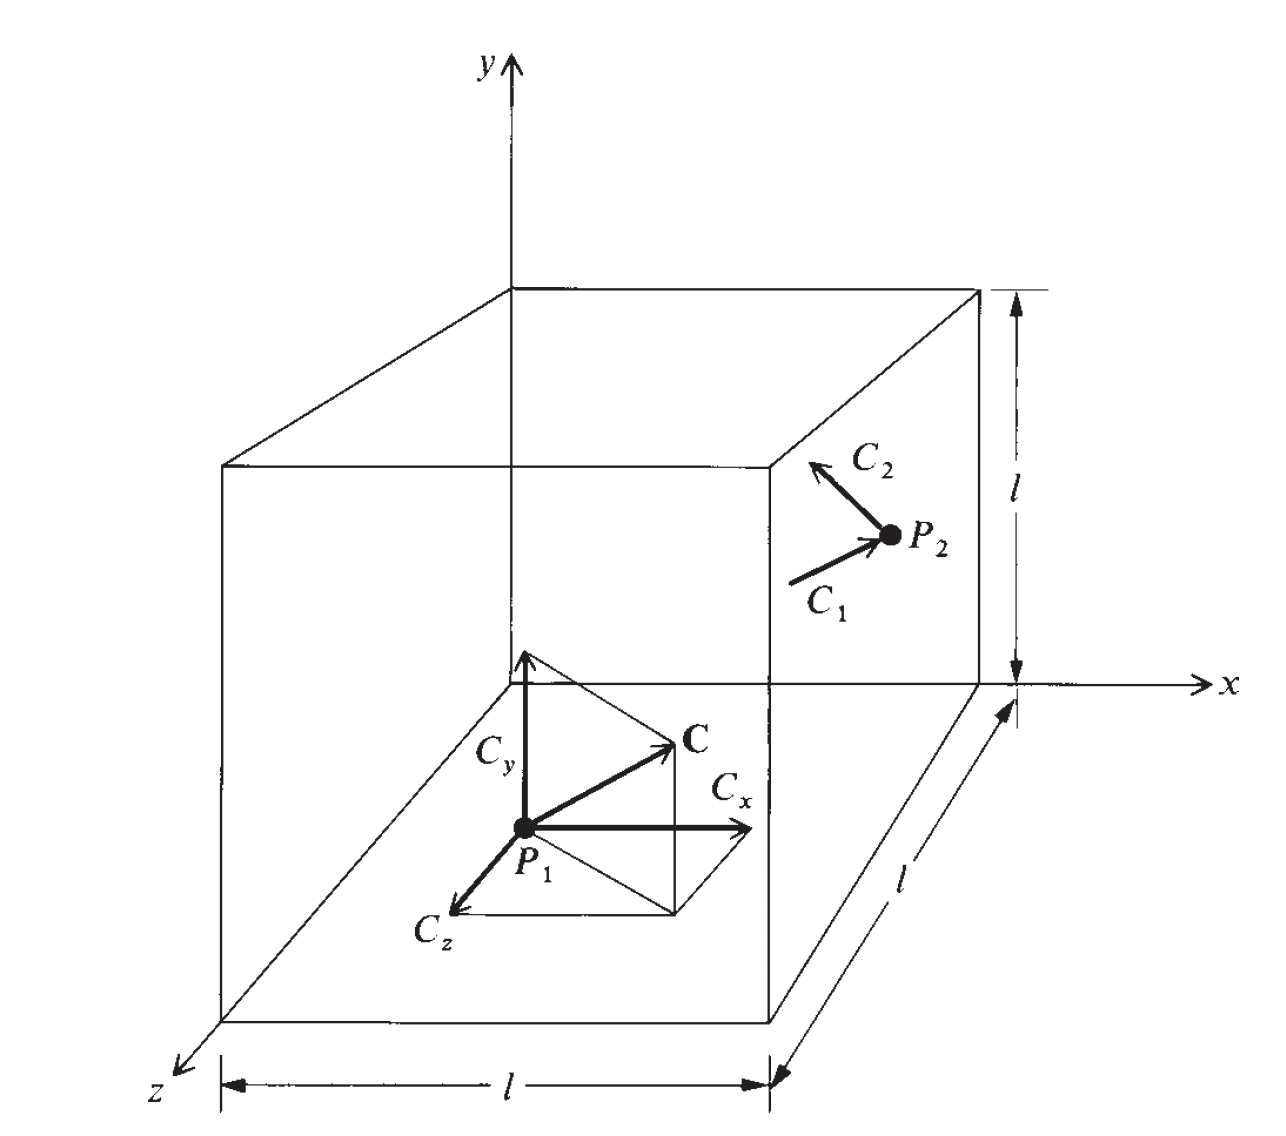
\includegraphics[width=0.45\textwidth]{box.png}
        \caption{Particle moving in a box; illustration of particle velocity components.}
    \end{figure}
\end{frame}

\begin{frame}
\frametitle{State equation: Perfect gases}
\begin{itemize}

    \item The goal is to derive the equation of state based on molecular collisions and motion.
    \item Assumes gas particles behave like "billiard balls" frequently colliding with neighboring particles.
    \item Single out a given gas particle at some instant and at some point P1.
  
\end{itemize}
\vskip-0.25cm
\begin{figure}
        \centering
        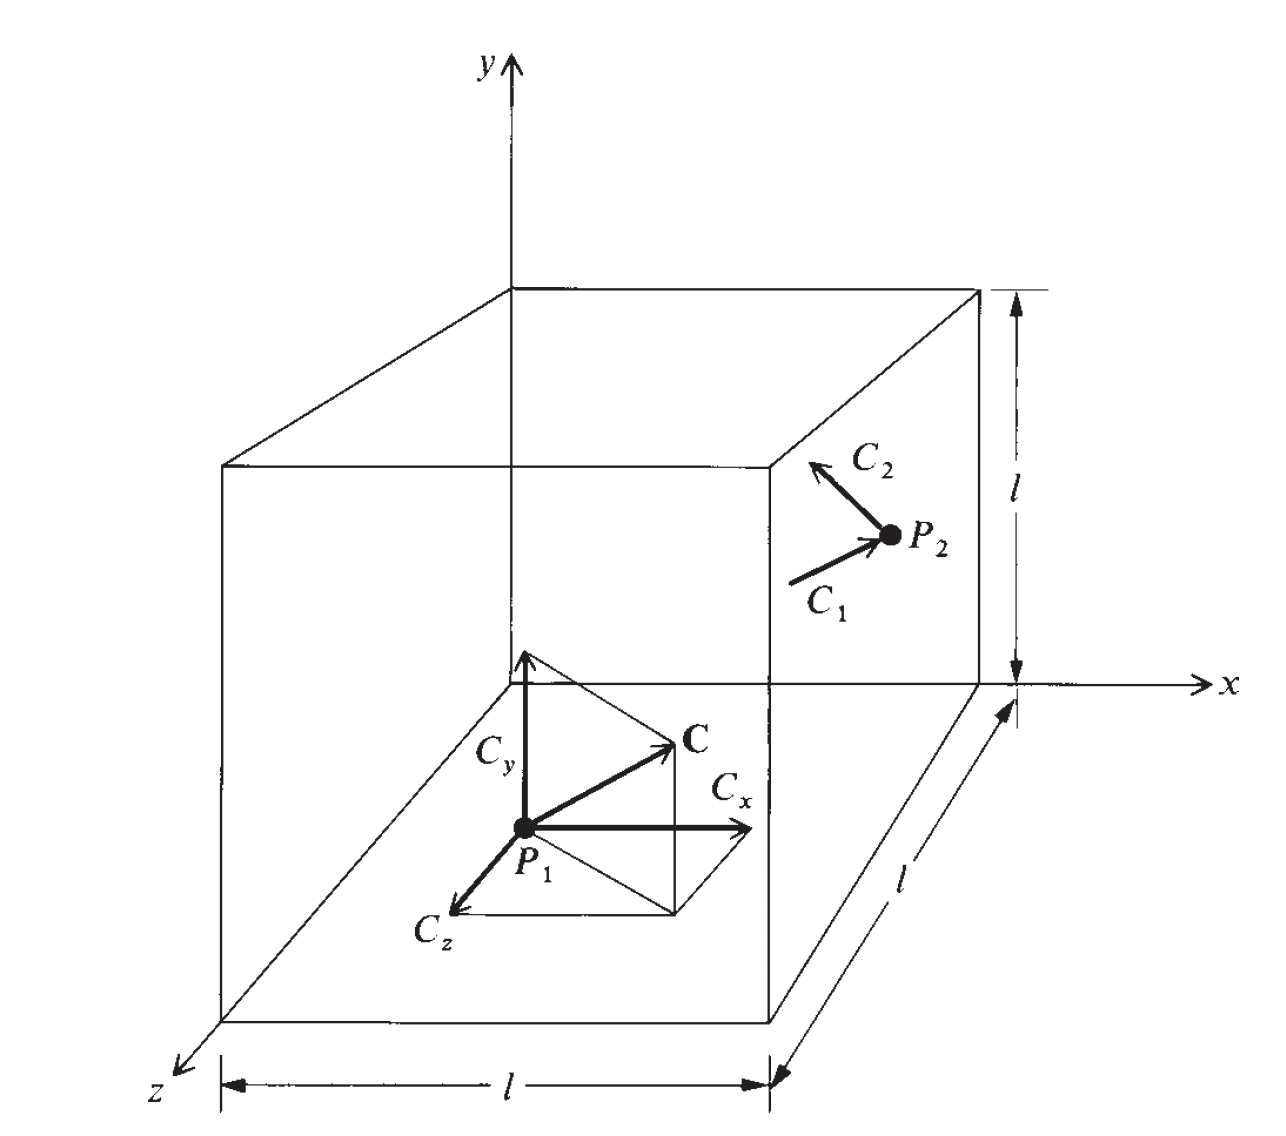
\includegraphics[width=0.45\textwidth]{box.png}
        \caption{Particle moving in a box; illustration of particle velocity components.}
    \end{figure}
\end{frame}

\begin{frame}
\frametitle{Box in Equilibrium}
\begin{itemize}

    \item Assume that the gas in the box
is in equilibrium. This implies that at any given point P$_1$ if a given particle with
velocity C$_1$ collides with another particle, causing a change in velocity, then there
is another collision between other particles in the same neighborhood, which
causes one of those other particles to have the velocity C$_1$ at point P$_1$.
  
\end{itemize}
\vskip-0.25cm
\begin{figure}
        \centering
        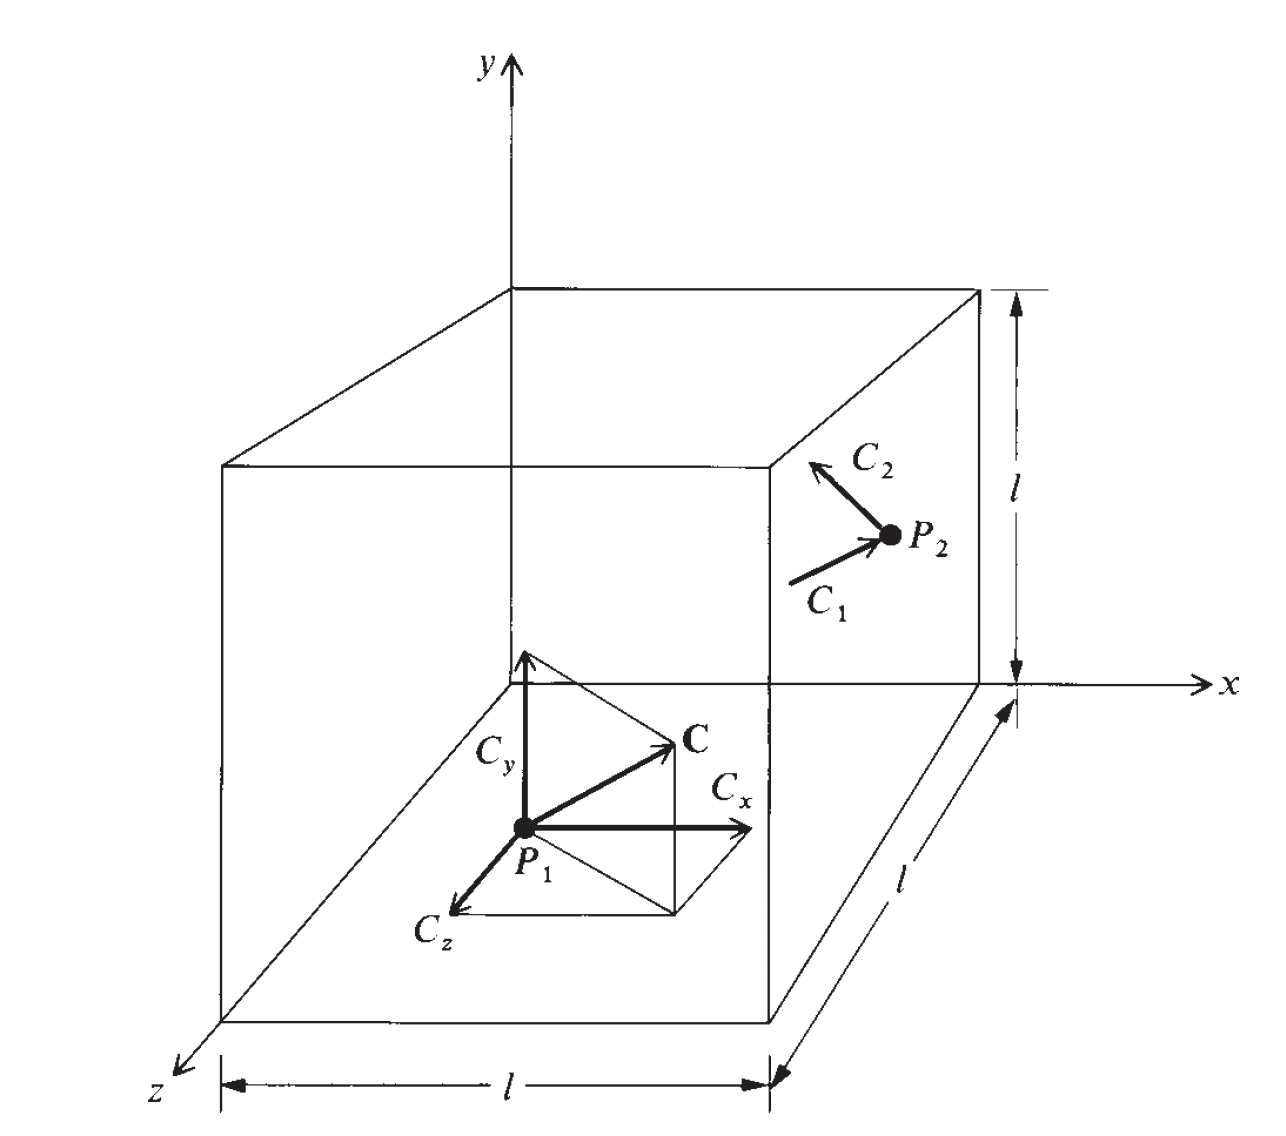
\includegraphics[width=0.45\textwidth]{box.png}
        \caption{Particle moving in a box; illustration of particle velocity components.}
    \end{figure}
\end{frame}

\begin{frame}
\frametitle{Particle Collisions and Equilibrium}
\begin{itemize}
\item This molecule can be regarded as carrying on
the motion of the original molecule just as if no collision had occurred.
\item The net result is as if the original particle continued at the velocity C$_1$. 
\item With this picture, we can visualize a particle traversing the box with a constant velocity in the x direction, given by Cx.
\item When the particle reaches the right face of the box, it is assumed to reflect from the surface at point P$_2$ specularly.
  
\end{itemize}
\end{frame}

\begin{frame}
\frametitle{Particle Traversal and Momentum Exchange}
\begin{itemize}

    \item The particle reflects specularly off the walls of the box.
    \item That is, if C$_1$ is the velocity just before impacting the surface at point P$_2$, and C$_2$ is the velocity immediate after impact, 
    $$
    \left|\boldsymbol{C}_1\right|=\left|\boldsymbol{C}_2\right|, C_{x_2}=-C_{x_1}, C_{y_2}=C_{y_1}
    $$
    \item Momentum change per collision in the $x$-direction: $\Delta p_x = 2mC_x$
    \item Collisions with the wall lead to a force exerted on the walls by particles, proportional to their velocity squared.
\end{itemize}
\end{frame}




\begin{frame}
\frametitle{Momentum Change Due to Collision}
\begin{itemize}
    \item When the particle collides with the wall perpendicular to the $x$-axis, it experiences a change in momentum.
    \item Before impact: velocity $C_{x1}$.
    \item After impact: velocity $C_{x2} = -C_{x1}$ (specular reflection).
    \item Change in momentum during collision:
    \[
    \Delta p_x = 2mC_x
    \]
    \item This occurs each time the particle reflects from the wall.
\end{itemize}
\end{frame}

\begin{frame}
\frametitle{Time Between Collisions}
\begin{itemize}
    \item The particle travels a distance $2l$ (back and forth) between successive collisions with the same wall.
    \item Time taken for a complete traversal (back and forth):
    \[
    t = \frac{2l}{C_x}
    \]
    \item Counting a complete traverse as going and coming to and from the right-hand face, the number of complete traverses per unit time is:
    \[
    \frac{C_x}{2l}
    \]
    \item Thus, the particle collides with the wall $\frac{C_x}{2l}$ times per second.
\end{itemize}
\end{frame}

\begin{frame}
\frametitle{Force Exerted by the Particle on the Wall}
\begin{itemize}
    \item The rate of change of momentum is equal to the force exerted on the wall.
    \item Momentum change per collision: $2mC_x$.
    \item Collisions per second: $\frac{C_x}{2l}$.
    \item  From Newton’s second law, the time rate of momentum change is equal to the force. Therefore, the force exerted by the particle on the wall:
    \[
    F_x = \frac{2mC_x \cdot C_x}{2l} = \frac{mC_x^2}{l}
    \]
\end{itemize}
\end{frame}

\begin{frame}
\frametitle{Pressure Exerted on the Wall}
\begin{itemize}
    \item Pressure is defined as force per unit area.
    \item Area of the wall: $l^2$.
    \item Pressure exerted by the particle on the wall:
    \[
    p_x = \frac{F_x}{l^2} = \frac{mC_x^2}{l^3} = \frac{mC_x^2}{V}
    \]
    where $V = l^3$ is the volume of the box.
\end{itemize}
\end{frame}

\begin{frame}
\frametitle{Extending to All Particles}
\begin{itemize}
    \item Now consider $N$ particles, each with different velocities $C_i = (C_{i,x}, C_{i,y}, C_{i,z})$.
    \item The pressure exerted by all particles in the $x$-direction:
    \[
    p_x = \frac{1}{V} \sum_{i=1}^{N} m_i C_{i,x}^2
    \]
    \item Similarly for the $y$ and $z$ directions:
    \[
    p_y = \frac{1}{V} \sum_{i=1}^{N} m_i C_{i,y}^2, \quad p_z = \frac{1}{V} \sum_{i=1}^{N} m_i C_{i,z}^2
    \]
\end{itemize}
\end{frame}

\begin{frame}
\frametitle{Total Pressure}
\begin{itemize}
    \item Total pressure is the sum of the pressures ($p_x$, $p_y$ and $p_z$) in all three directions:
    \[
    p = \frac{1}{3V} \sum_{i=1}^{N} m_i (C_{i,x}^2 + C_{i,y}^2 + C_{i,z}^2) = \frac{1}{3V} \sum_{i=1}^{N} m_i C_i^2
    \]
    where $C_i^2 = C_{i,x}^2 + C_{i,y}^2 + C_{i,z}^2$ is the square of the velocity magnitude for particle $i$.
\end{itemize}
\end{frame}

\begin{frame}
\frametitle{Kinetic Energy of the System}
\begin{itemize}
    \item The total translational kinetic energy of the system is:
    \[
    E_{\text{trans}} = \frac{1}{2} \sum_{i=1}^{N} m_i C_i^2
    \]
    \item Using this expression, we can rewrite the pressure as:
    \[
    pV = \frac{2}{3} E_{\text{trans}}
    \]
    \item This is a key relation in kinetic theory, linking macroscopic pressure and volume with microscopic kinetic energy.
    \item It can only be related to temperature through classical thermodynamics
because T is a variable that originated with classical thermodynamics.
\end{itemize}
\end{frame}

\begin{frame}
\frametitle{Relation to Temperature}
\begin{itemize}
    \item The ideal gas law states that:
    \[
    pV = nRT
    \]
    where $n$ is the number of moles, and $R$ is the universal gas constant.
    \item From kinetic theory:
    \[
    pV = \frac{2}{3} E_{\text{trans}}
    \]
    \item We see that the theoretical state equation formula and the empirical equation are identical if we take
    \[
    \boxed{E_{\text{trans}} = \frac{3}{2} nRT}
    \]
\end{itemize}
\end{frame}

\begin{frame}
\frametitle{Mean Kinetic Energy per Particle}
\begin{itemize}
    \item The total kinetic energy can be written as:
    \[
    E_{\text{trans}} = N \cdot \left( \frac{1}{2} m \bar{C^2} \right)
    \]
    where $\bar{C^2}$ is the mean square velocity of the particles.
    \item Equating this with the expression from temperature:
    \[
    \frac{3}{2} nRT = N \cdot \frac{1}{2} m \bar{C^2}
    \]
    \item This leads to the mean square velocity:
    \[
   \boxed{\bar{C^2} = \frac{3RT}{M}}
    \]
    where $M$ is the molar mass.
\end{itemize}
\end{frame}



\begin{frame}
\frametitle{Molecular Speeds and Kinetic Theory}
\begin{itemize}
    \item The mean square velocity is defined as:
    \[
    \bar{C}^2 = \frac{\sum_i m_i C_i^2}{\sum_i m_i}
    \]
    \item Relating pressure to the mean square velocity:
    \[
    \frac{p}{\rho} = \frac{1}{3} \bar{C}^2
    \]
    \item The root mean square (rms) molecular velocity is:
    \[
    \bar{C} = \sqrt{3RT}
    \]
\end{itemize}
\end{frame}

\begin{frame}
\frametitle{Introduction to Velocity Distribution Functions}
 \begin{figure}
        \centering
        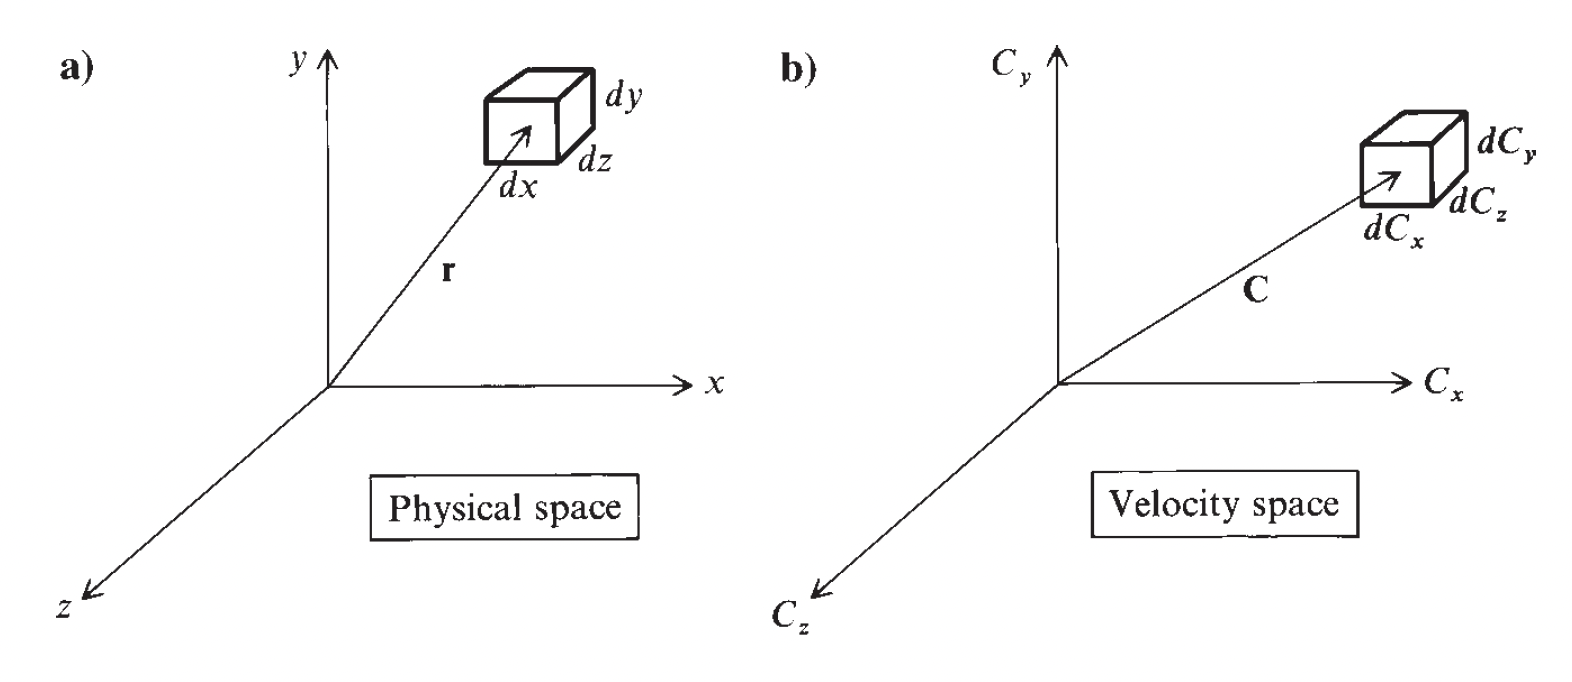
\includegraphics[width=0.85\textwidth]{phase_space.png}
        \caption{Illustration of volume elements in physical and velocity spaces.}
    \end{figure}
\begin{itemize}
    \item A system of $N$ particles is distributed throughout physical space.
    \item The instantaneous location of each particle is described by the vector $\mathbf{r}$ in the $x$-$y$-$z$ space.
    \item Each particle has a velocity $\mathbf{C}$, described in the $C_x$-$C_y$-$C_z$ velocity space.
\end{itemize}
\end{frame}

\begin{frame}
\frametitle{Velocity Distribution in Space and Velocity}
\begin{itemize}
    \item Thus, at any instant, the system can be represented by a cloud of points in both physical space and velocity space.
    \item Consider a point in physical space, $\mathbf{r}$, and a unit volume in velocity space centered around $\mathbf{C}$.
    \item The distribution function $\hat{f}(\mathbf{r}, \mathbf{C})$ is defined as the number of particles per unit volume of physical space at $\mathbf{r}$, with velocities in the unit volume of velocity space centered at $\mathbf{C}$.
    \item Mathematically, $\hat{f}(x, y, z, C_x, C_y, C_z)$ represents the number of particles located between $x$ and $x + dx$, $C_x$ and $C_x + dC_x$, etc.
\end{itemize}
\end{frame}

\begin{frame}
\frametitle{Velocity Distribution Function}
\begin{itemize}
    \item The distribution function $\hat{f}(\mathbf{r}, \mathbf{C}) dV_{\text{phys}} dV_{\text{vel}}$ gives the number of particles in a small physical volume $dV_{\text{phys}} = dx\,dy\,dz$ and a small velocity volume $dV_{\text{vel}} = dC_x\,dC_y\,dC_z$.
    \item The system consists of particles moving continuously, with velocities changing due to collisions.
    \item In a nonequilibrium gas, the number of particles within the element $dx\,dy\,dz$ varies with both position $\mathbf{r}$ and time $t$.
\end{itemize}
\end{frame}

\begin{frame}
\frametitle{Key Concept: Distribution Function}
\begin{itemize}
    \item The distribution function is a key concept in classical kinetic theory.
    \item Integrating $\hat{f}(\mathbf{r}, \mathbf{C})$ over all space and velocities gives the total number of particles in the system:
    \[
    \int_{-\infty}^{\infty}  \hat{f}(x, y, z, C_x, C_y, C_z) dx\,dy\,dz\,dC_x\,dC_y\,dC_z = N
    \]
    \item sometimes a different notation is used whereby
        \[
    \int_{-\infty}^{\infty} n \, f(x, y, z, C_x, C_y, C_z) dx\,dy\,dz\,dC_x\,dC_y\,dC_z = N
    \]
    \item hence
            \[
    \int_{-\infty}^{\infty}  f(x, y, z, C_x, C_y, C_z) \; dx\,dy\,dz\,dC_x\,dC_y\,dC_z = 1
    \]
\end{itemize}
\end{frame}

\begin{frame}
\frametitle{Application of Distribution Functions}
\begin{itemize}
    \item The distribution function is used to compute average values of any physical quantity $Q$, which is a function of space and velocity.
    \item For example, the average value of $Q(\mathbf{r}, \mathbf{C})$ is given by:
    \[
    \bar{Q} = \frac{1}{N} \int_{-\infty}^{\infty}  Q(x, y, z, C_x, C_y, C_z) \; n \, f ({\bf r}, {\bf C})\; dx\,dy\,dz\,dC_x\,dC_y\,dC_z
    \]
\end{itemize}
\end{frame}

\begin{frame}
\frametitle{Physical Meaning of $f(\mathbf{r}, \mathbf{C})$}
\begin{itemize}
    \item $f(\mathbf{r}, \mathbf{C})$ tells us how particles are distributed in physical and velocity space at any given time.
    \item For a nonequilibrium gas, $f(\mathbf{r}, \mathbf{C})$ changes with time and space due to particle collisions and external forces.
    \item The velocity distribution function is crucial for calculating macroscopic properties such as pressure, temperature, and density.
\end{itemize}
\end{frame}

\begin{frame}
\frametitle{Using Distribution Functions in Kinetic Theory}
\begin{itemize}
    \item By knowing $f(\mathbf{r}, \mathbf{C})$, we can compute:
    \begin{itemize}
        \item Average velocity components.
        \item Energy distribution.
        \item Fluxes and transport properties.
    \end{itemize}
    \item Distribution functions form the foundation of more advanced kinetic theory models such as the Boltzmann equation.
\end{itemize}
\end{frame}

\begin{frame}
\frametitle{Notes on the distribution function: Basics}
The distribution function \( f(C_i) \) gives the fraction of molecules in class \( C_i \), that is, the fraction with velocity in the range \( (C_i, C_i + dC_i) \). This function is fundamental in kinetic theory to describe how molecules are distributed in terms of their velocities.\\
\begin{itemize}

    \item 
     $$
    f(C_i) dV_C     
    $$
    fraction of molecules in class, $C_i$, i.e., fraction with velocity in the range ($C_i, C_i+d C_i$):
   \item This definition can be thought as the conditional probability of the previously defined distribution function. This gives the probability at one position.
   
\end{itemize}

\end{frame}
\begin{frame}{Coordinate Systems}
\begin{itemize}

  \item Representation of d $V_C$ depends on the coordinate basis chosen in the {\bf velocity space}.
    $C_i$ is a vector $C_i = (C_1, C_2, C_3)$
    $$
    dV_C = dC_1 \, dC_2 \, dC_3 \quad \textit{Cartesian}
    $$
    $$
     dV_C = C^2 dC \sin{\theta} \, d {\theta} \, d {\phi} \quad \textit{Spherical Coordinates}
    $$
\end{itemize}
\begin{figure}
        \centering
        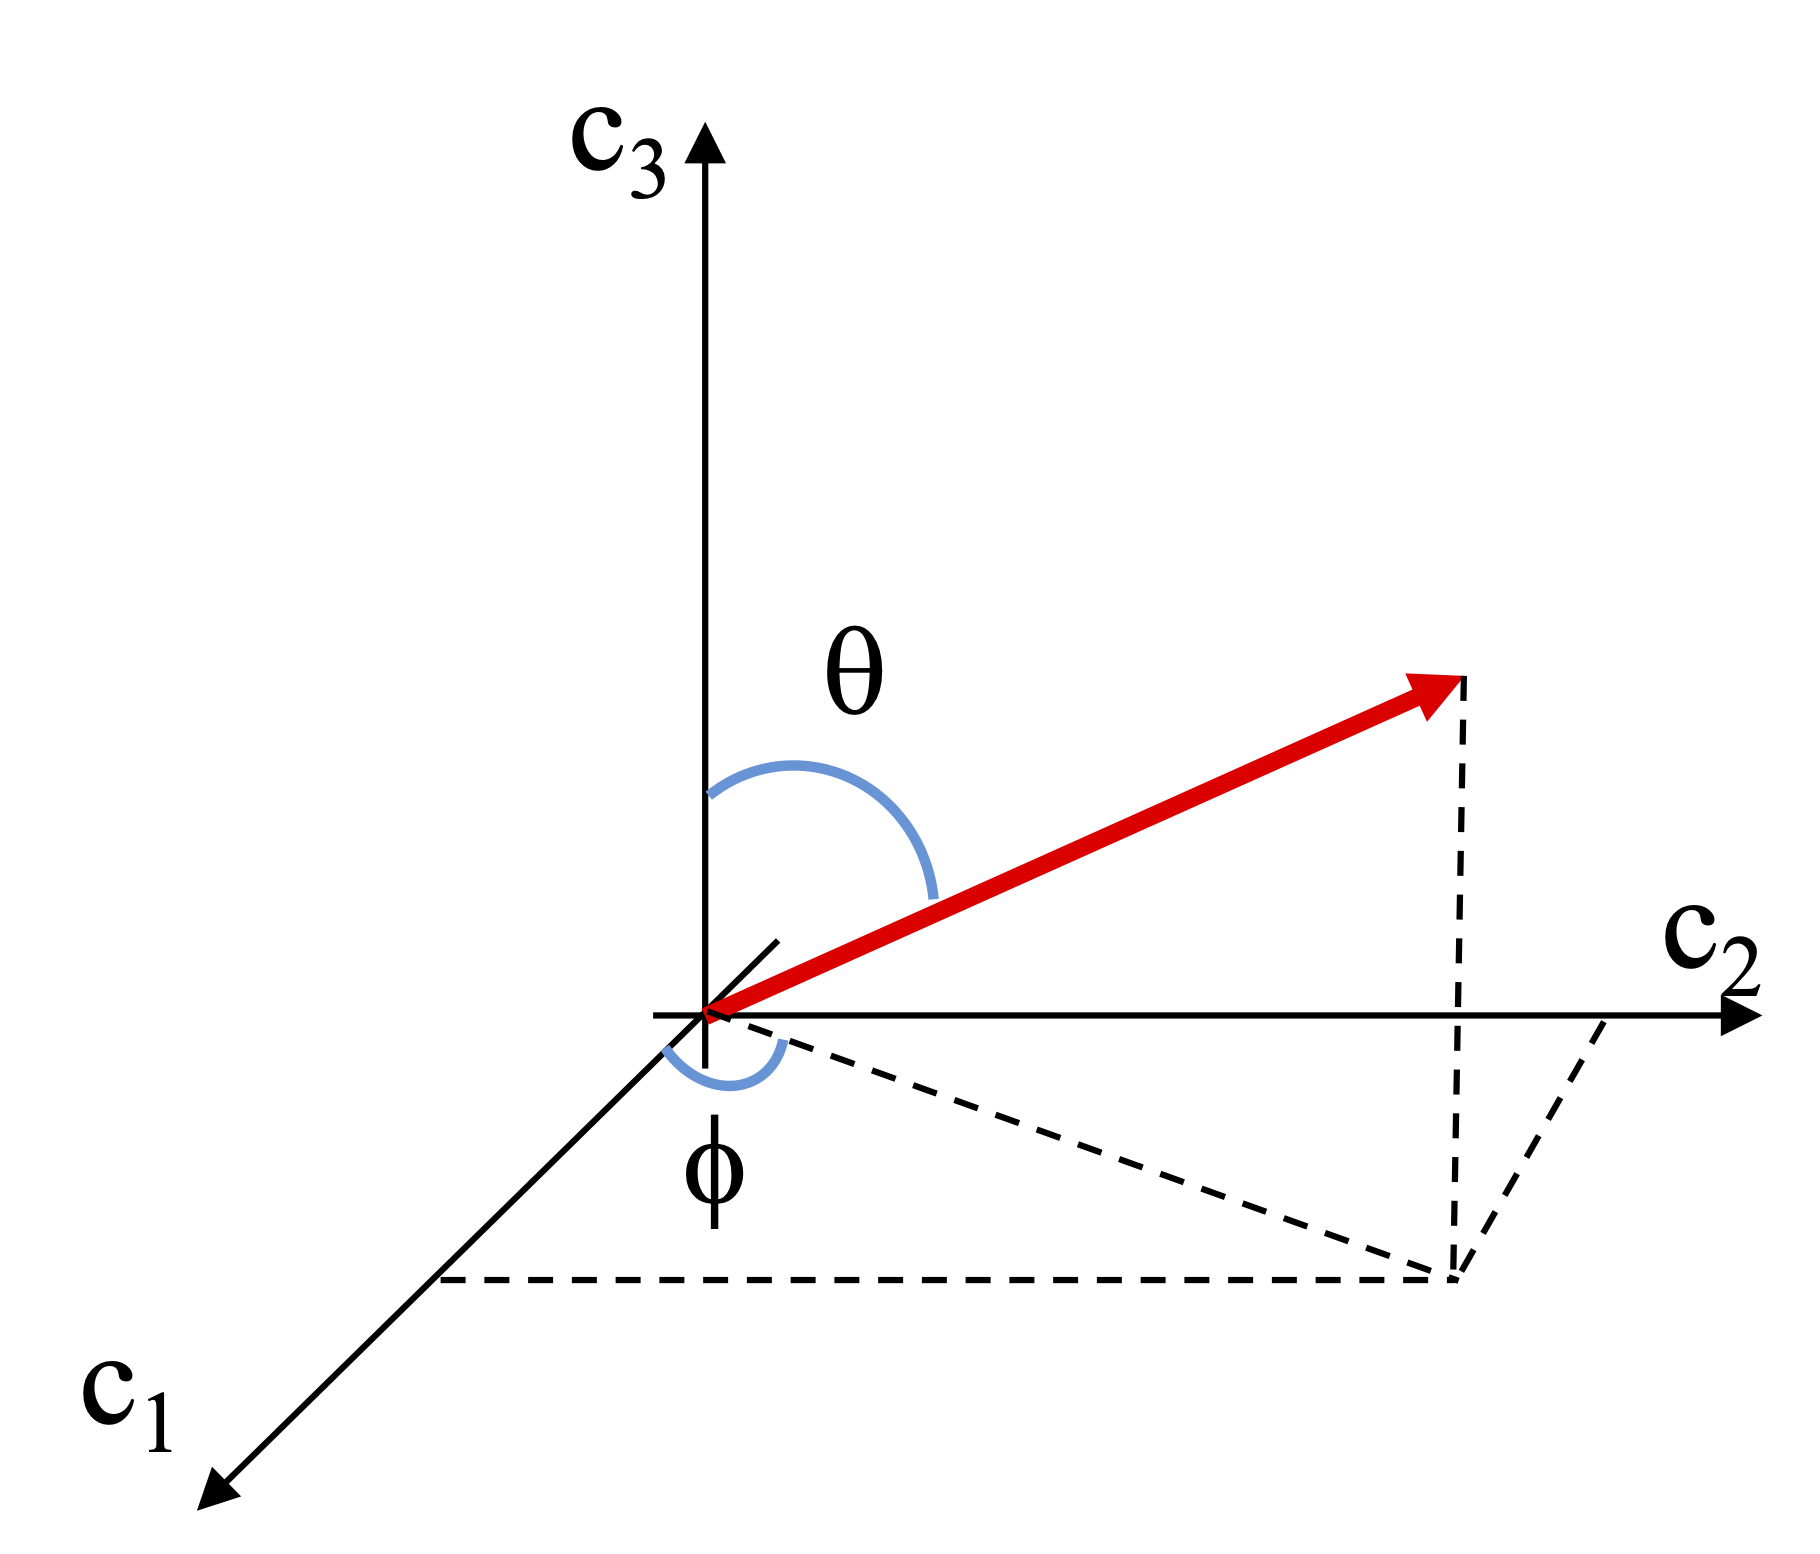
\includegraphics[width=0.45\textwidth]{coord.png}
        \caption{Cartesian and Spherical Coordinates}
    \end{figure}
\end{frame}

\begin{frame}
\frametitle{Notes on the distribution function: Basics}
\begin{itemize}

    \item {\bf Number flux  of molecules}
    $$
    \phi^{n}_k = \frac{\# \textit{of molecules}}{\textit{time} \; \textit{area}}
    $$
    \item {\bf Differential flux of molecules} traveling in direction k:
    $$
    d^{(3)} \phi^{n}_k = n \left( C_i \cdot \hat{i}_k \right) \; f (C_i) \; dV_C
    $$
    \item 
    e.g., differential flux  in $x_2$ direction $ d^{(3)} \phi^{n}_2 = n \; C_2  \; f (C_i) \; dV_C$
\end{itemize}
\vskip0.5cm
Note that $C_2$ is the x-component of velocity $C_i$, and $d^{(3)} \phi^{n}_2$ is the differential flux of class $C_i$ in the $x_2$ direction. 

\end{frame}

\begin{frame}
\frametitle{Notes on the distribution function: Basics}
\begin{itemize}
    \item  One can construct differential flux of momentum and energy.
    \item The number flux and energy flux are vectors. The direction is the direction where the flux occurs.
    \item Momentum flux is a tensor: one direction is the direction components, and the other is the direction in which this vector quantity is being transported. 

\end{itemize}


\end{frame}

\begin{frame}
\frametitle{Notes on the distribution function: Basics}

\begin{itemize}
\item Example 1: Energy: Differential kinetic energy flux in x$_2$ direction being transported by molecules of class $C_i$; C$_2$  the C$_i$ component in x-2 direction
 
   $$
    d^{(3)} \phi^{\epsilon}_2 = \left(\frac{1}{2} m \, C^2_i\right) \; n\;  C_2 \; f (C_i) \; dV_C 
    $$
    
\item Example 2: Differential Momentum flux: 
    $$
   d^{(3)} \phi^{p}_{1,2} = \left(m \,  C_1 \right) \; n\; C_2 \; f (C_i) \; dV_C 
   $$
    Differential x1-momentum flux  in x$_2$ direction being transported by molecules of class $C_i$; C$_2$ os the C$_i$ component in x-2 direction
    
\end{itemize}


\end{frame}

\begin{frame}
\frametitle{Collisions and Velocity Distribution}
\begin{figure}
        \centering
        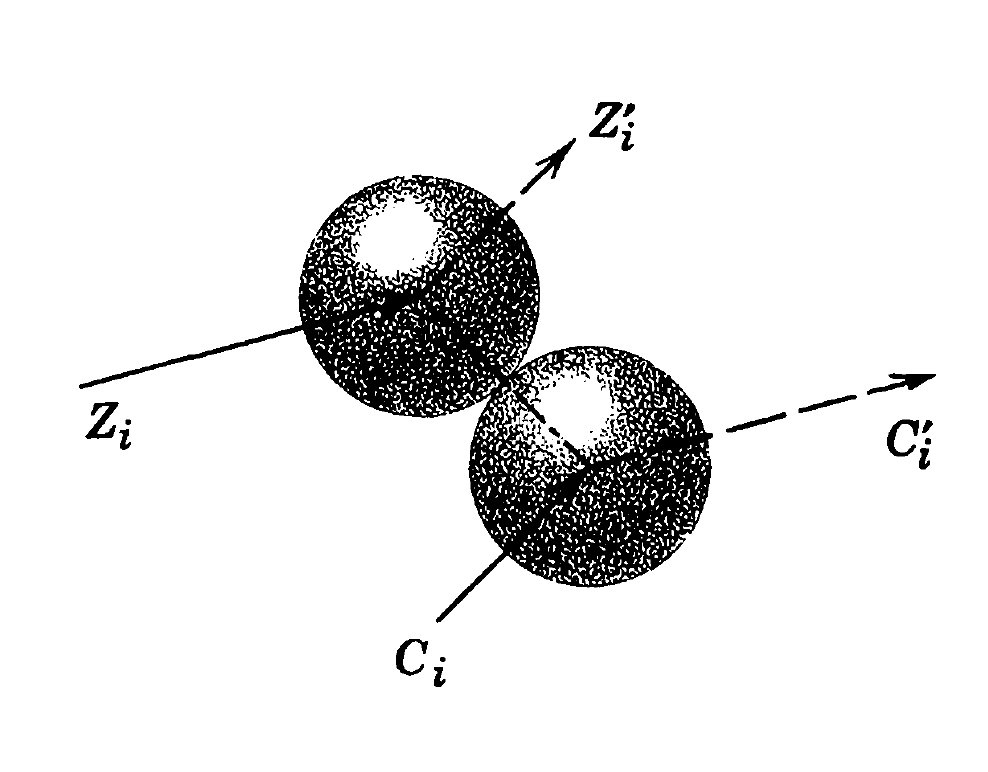
\includegraphics[width=0.4\textwidth]{collisions.png}
        \caption{Cartesian and Spherical Coordinates}
    \end{figure}
\begin{itemize}
    \item Collisions are constant and alter the velocity distribution of molecules.
    \item Pre- and post-collision velocities are different:
    \[
    (C_i, Z_i) \longrightarrow (C'_i, Z'_i)
    \]
    \item The equilibrium distribution is the one that remains unchanged even as collisions continue to occur.
\end{itemize}
\end{frame}

\begin{frame}
\frametitle{Collision Rate Definition}
\begin{itemize}
    \item The collision rate between molecules of type A and type B is defined as:
    \[
    Z_{\text{AB}} = \frac{\text{Number of collisions}}{\text{Time} \times \text{Volume}}
    \]
    \item This rate helps quantify how frequently collisions occur between different molecular species.
\end{itemize}
\end{frame}

\begin{frame}
\frametitle{Hard Sphere (HS) Model}
\begin{itemize}
    \item In the HS model, molecules are treated as hard spheres, analogous to billiard balls.
    \item Molecules A and B have masses $m_A$ and $m_B$, and diameters $d_A$ and $d_B$, respectively.
    \item Relative velocity between A and B is defined as:
    \[
    g_i = Z_i - C_i
    \]
    \item A collision occurs if the relative distance between A and B satisfies:
    \[
    b \leq \frac{d_A + d_B}{2} = d_{AB}
    \]
    where $d_{AB}$ is the sum of the radii of A and B.
\end{itemize}
\end{frame}

\begin{frame}
\frametitle{Collisions and Velocity Distribution}
\begin{figure}
        \centering
        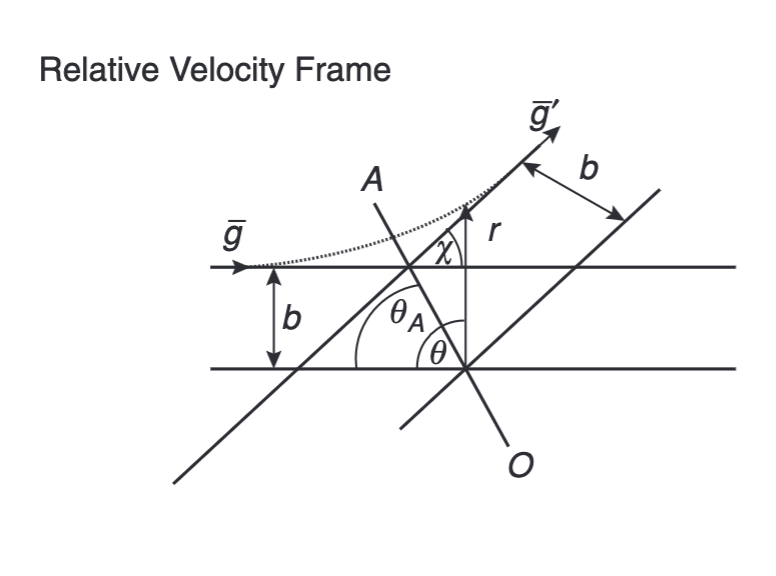
\includegraphics[width=0.85\textwidth]{collision_relative.png}
        \caption{Cartesian and Spherical Coordinates}
    \end{figure}
    \end{frame}
\begin{frame}
\frametitle{Collision Cross Section}
\begin{itemize}
    \item A collision occurs if the center of molecule B enters a sphere of radius $d_{AB}$ around molecule A.
    \item The cross-sectional area of this sphere is the target area for the collision.
    \item The total collision cross section, $\sigma_t$, for hard spheres is:
    \[
    \sigma_t = \pi d_{AB}^2
    \]
    \item A collision will occur if the relative velocity $g_i$ is directed within this area.
\end{itemize}
\end{frame}

\begin{frame}
\frametitle{Improved Models: Variable Hard Sphere (VHS)}
\begin{itemize}
    \item The Hard Sphere (HS) model, while conceptually simple, is not always sufficiently accurate.
    \item The VHS model improves accuracy by making the collision cross section a function of the relative speed $g$:
    \[
    \sigma_t = \sigma(g)
    \]
    \item This is widely used in aerodynamic calculations, while more complex models are applied in chemistry and physics.
\end{itemize}
\end{frame}

\begin{frame}
\frametitle{Total Cross Section}
\begin{itemize}
    \item The total cross section integrates over all possible collision outcomes.
    \item Includes:
    \begin{itemize}
        \item Elastic collisions (no change in internal energy).
        \item Inelastic collisions and chemical reactions.
    \end{itemize}
    \item Elastic collisions are simpler as they preserve the kinetic energy.
\end{itemize}
\end{frame}

\begin{frame}
\frametitle{Elastic Collisions}
\begin{itemize}
    \item Elastic collisions are particularly important in many gas dynamic and kinetic theory calculations.
    \item Elastic collisions: no change in internal energy, and total kinetic energy remains constant.
    \item In an elastic collision:
    \[
    (C_i, Z_i) \longrightarrow (C'_i, Z'_i)
    \]
    where total kinetic energy before and after the collision is conserved.
    \item Elastic collisions change the direction of the relative velocity vector, but not the magnitude
\end{itemize}
\end{frame}

\begin{frame}
\frametitle{Elastic Collisions}
\begin{figure}
        \centering
        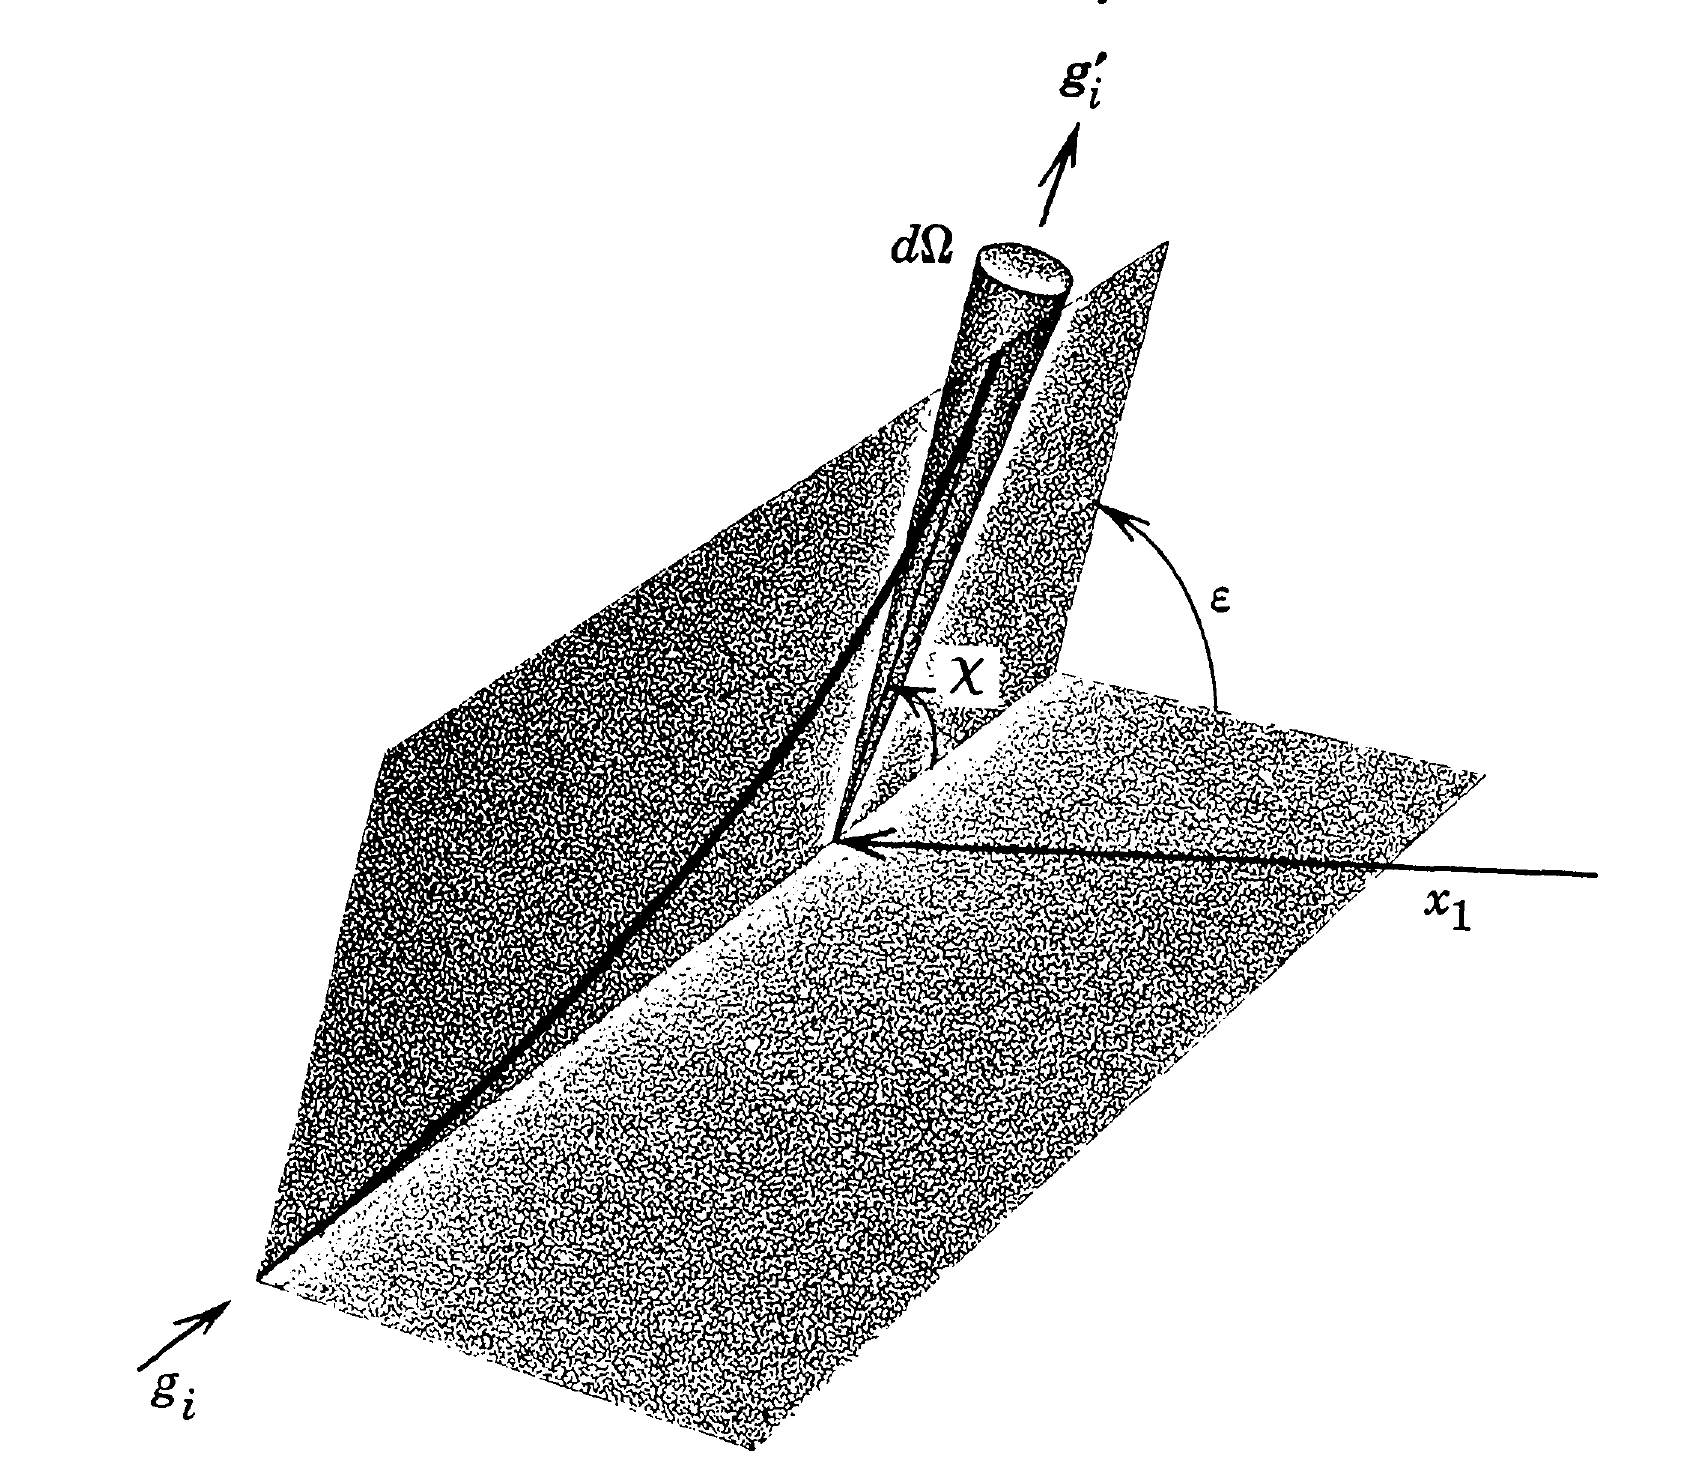
\includegraphics[width=0.55\textwidth]{collision_elastic.png}
        \caption{Collision: Spherical Coordinates}
    \end{figure}
\begin{itemize}
    \item The scattering can be specified by the polar angles $\chi$ and $\epsilon$, that indicate the orientation of $g'_i$ relative to  $g_i$
\end{itemize}
\end{frame}

\begin{frame}
\frametitle{Elastic Collisions}
\begin{itemize}
    \item The differential scattering solid angle corresponding variations in polar angle $(\chi)$, and azimuthal angle $\epsilon$ is given by
    $$
    d \Omega = sin \chi d \chi d\epsilon
    $$
\end{itemize}
\begin{figure}
        \centering
        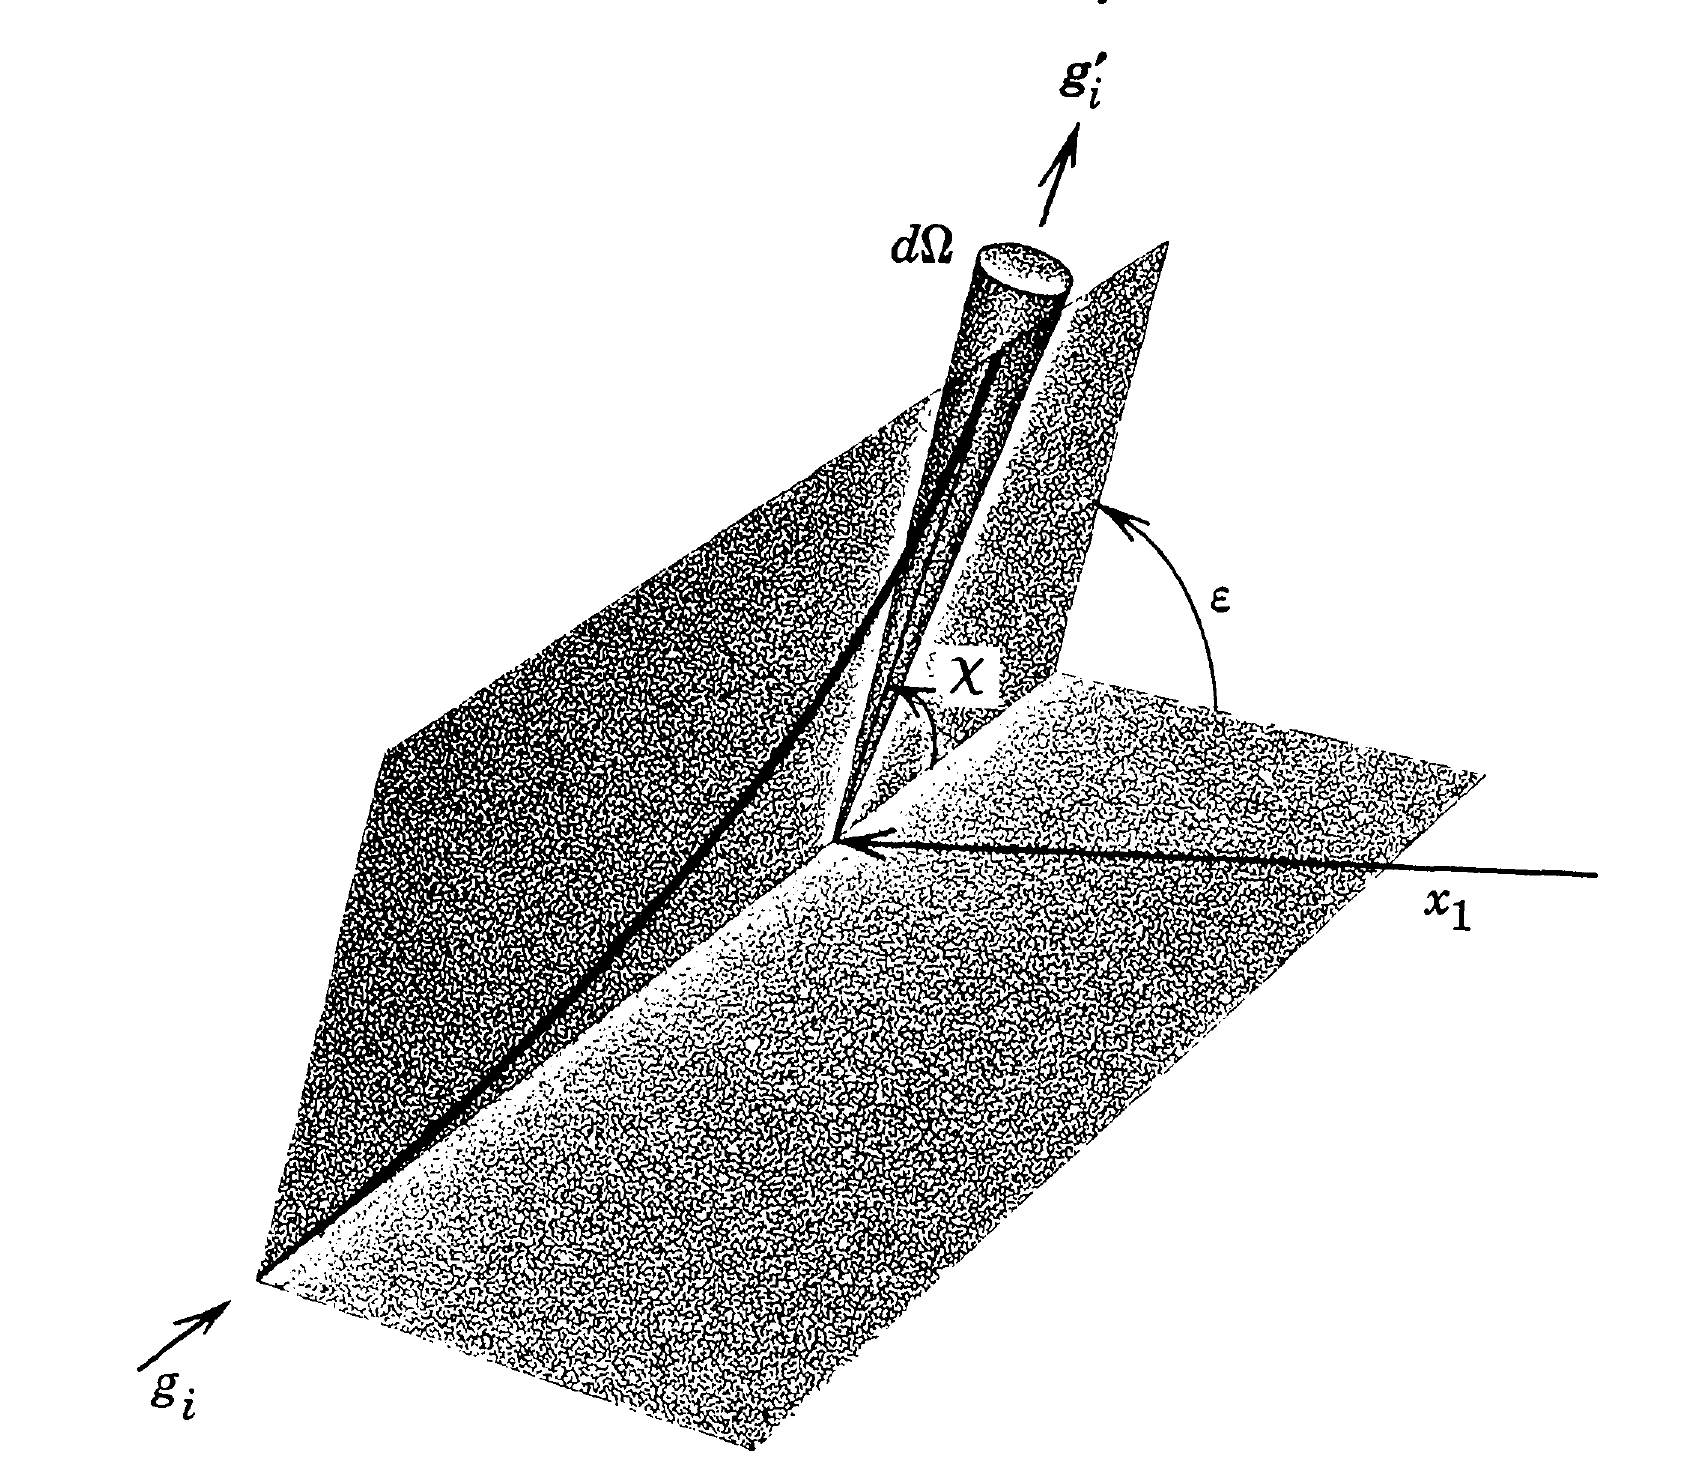
\includegraphics[width=0.5\textwidth]{collision_elastic.png}
        \caption{Collision: Spherical Coordinates}
    \end{figure}

\end{frame}

\begin{frame}
\frametitle{Differential Cross Section}
\begin{itemize}
    \item The differential cross-section 
    $$
    \left(\frac{d \sigma}{d \Omega}\right)
    $$
  corresponds to the probability that scattering occurs into d$\Omega$, i.e., that the orientation of $g\prime_i$ specified by $\epsilon$ and  $\chi$ is within d$\Omega$.
\end{itemize}
\end{frame}

\begin{frame}
\frametitle{Total Cross Section}
\begin{itemize}
    \item The \emph{total cross section} $\sigma_T$ integrates the differential cross section over all possible scattering directions:
    \[
    \sigma_T = \int_{\Omega} \frac{d\sigma}{d\Omega} \, d\Omega = \int_0^{2\pi} \int_0^{\pi} \frac{d\sigma}{d\Omega} \sin \chi \, d\chi \, d\epsilon
    \]
    \item This gives the overall likelihood of a collision, including elastic, inelastic, or reactive collisions.
\end{itemize}
\end{frame}

\begin{frame}
\frametitle{Simplified Cases}
\begin{itemize}
    \item If scattering is azimuthally symmetric (independent of \( \epsilon \)):
    \[
    \sigma_T = 2\pi \int_0^{\pi} \left( \frac{d\sigma}{d\Omega} \right) \sin \chi \, d\chi
    \]
    \item For isotropic scattering (independent of both \( \chi \) and \( \epsilon \)):
    \[
    \sigma_T = 4\pi \left( \frac{d\sigma}{d\Omega} \right)
    \]
    \item Hard spheres are isotropic scatterers, and their total cross section is:
    \[
    \sigma_T = \pi d_{AB}^2
    \]
\end{itemize}
\end{frame}

\begin{frame}{Collision Frequency}
The collision frequency, $\Theta$, is defined as the number of collisions per unit time experienced by each particle.
\begin{figure}
        \centering
        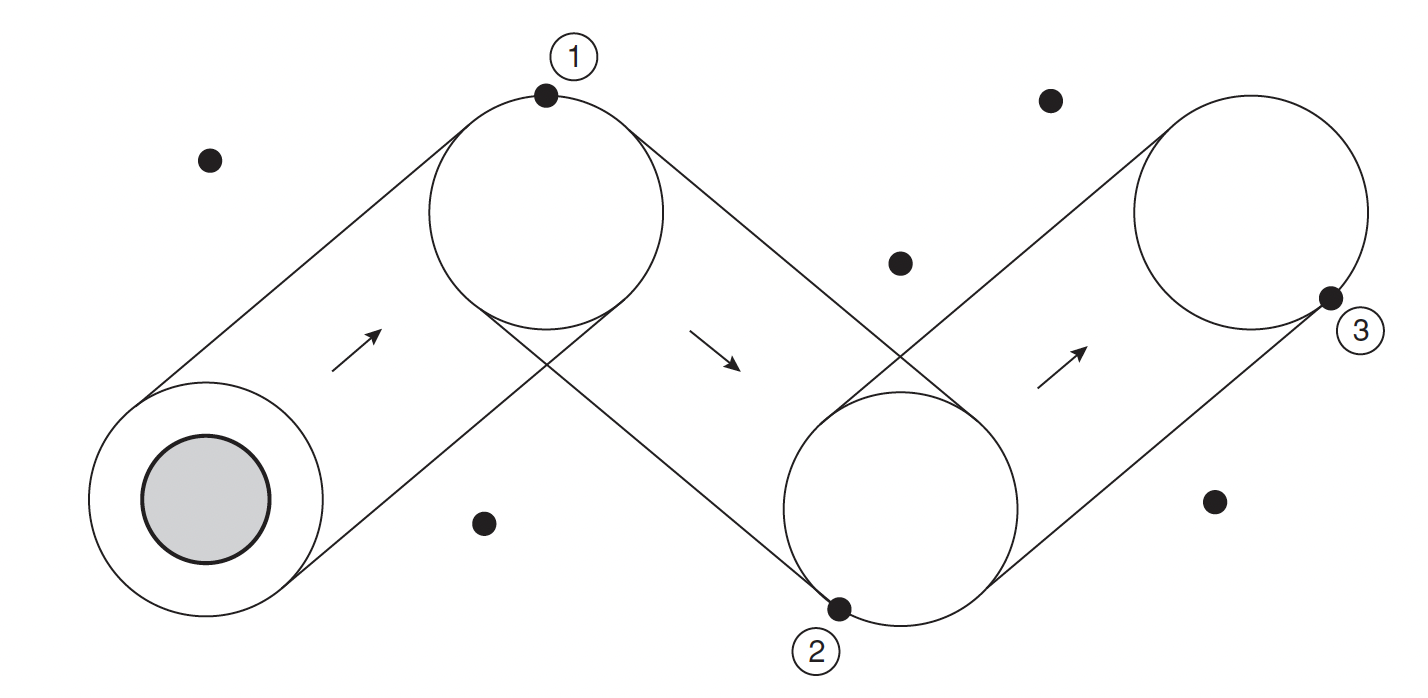
\includegraphics[width=0.85\textwidth]{collision_freq.png}
        \caption{Collisions of 1 B particle with many A particles}
    \end{figure}    
\end{frame}



\begin{frame}
\frametitle{Collision Frequency}
\begin{itemize}
    \item Consider a {\bf single} molecule B moving with velocity \( g_i \) relative to molecule A of class C$_i$. 
    \item The particle B sweeps out a volume in the unit time, dt:
    \[
    dV = g \, dt \, \left( \frac{d\sigma}{d\Omega} \right) d\hat{\Omega}
    \]
    \item The number of A molecules of class C$_i$ in this volume is:
    \[
    n_A f_A(C_i) \, dV_c \cdot g \, dt \, \left( \frac{d\sigma}{d\Omega} \right) d\hat{\Omega}
    \]
    \item Differential collision frequency for this B molecule of class Z$_i$:
    \[
    d\Theta_{BA} = n_A f_A(C_i) \, dV_c \, g \,  \left( \frac{d\sigma}{d\Omega} \right) d\hat{\Omega}
    \]
\end{itemize}
\end{frame}

\begin{frame}
\frametitle{Total Collision Rate}
That is the number of collisions between A and B particles in the unit time.
\begin{itemize}
    \item But there are  \( n_B f_B(Z_i) \, dV_Z \) B molecules of class Z$_i$.
    \[
    d^{(8)}Z_{BA} = d^{(8)}Z_{AB}= n_A f_A(C_i) \, dV_c \, n_B f_B(Z_i) \, dV_Z \, g \left( \frac{d\sigma}{d\Omega} \right) d\hat{\Omega}
    \]
    \item Integrating over all solid angles \( d\hat{\Omega} \):
    \[
    d^{(6)}Z_{AB} = n_A f_A(C_i) \, dV_c \, n_B f_B(Z_i) \, dV_Z \, g \, \sigma_T
    \]
    \item Where \( \sigma_T \) is the total cross section.
\end{itemize}
\end{frame}
\begin{frame}
\frametitle{Maxwellian Distribution}
The goal of this section is to derive an expression for the Maxwellian velocity distribution.
\begin{itemize}
    \item Collisions deplete particles from some velocity class and replenish others.
    \item Replenishing rates are easier to handle by considering **inverse collisions**.
    \item Direct collision: \( (C_i, Z_i) \to (C'_i, Z'_i) \) (depleting).
    \item Inverse collision: \( (C'_i, Z'_i) \to (C_i, Z_i) \) (replenishing).
    \item Both direct and inverse collisions must be considered to calculate the rate of change in the velocity distributions.
\end{itemize}
\end{frame}

\begin{frame}{Rates for Direct and Inverse Collision}
    \begin{itemize}
    \item Direct collisions (\( (C_i, Z_i) \to (C'_i, Z'_i) \) (depleting).)
    \[
    d^{(8)}Z_{AB}= n_A \, n_B f_A(C_i)   f_B(Z_i) \, \, g \left( \frac{d\sigma}{d\Omega} \right)    d\hat{\Omega} dV_c dV_Z
   \]
    \item Inverse collision: \( (C'_i, Z'_i) \to (C_i, Z_i) \) (replenishing). 
      \[
    d^{(8)}Z^\prime_{AB}= n_A \, n_B f_A(C^\prime_i)   f_B(Z^\prime_i) \, \, g^\prime \left( \frac{d\sigma^\prime}{d\Omega} \right)    d\hat{\Omega} dV_c dV_Z
    \]
    \item net contribution
    \[  
    \frac{\partial}{\partial t} \left[ n_A f_A(C_i) dV_c \right]_{\text{colls}} = \] \\ 
    \[
    n_A \, n_B \left[f_A(C^\prime_i)   f_B(Z^\prime_i) - f_A(C_i)   f_B(Z_i)\right]\, \, g\left( \frac{d\sigma}{d\Omega} \right)    d\hat{\Omega} dV_c dV_Z
    \]
\end{itemize}
\end{frame}

\begin{frame}
\frametitle{Change in Particle Distribution}
\begin{itemize}
    \item The change in the number of particles in velocity class \( C_i \) due to collisions is:
    \[
    \frac{\partial}{\partial t} \left[ n_A f_A(C_i) dV_c \right]_{\text{colls}} = 
    \]
    \[
    n_A n_B \int_{V_z} \int_{\Omega} \left[ f_A(C_i') f_B(Z_i') - f_A(C_i) f_B(Z_i) \right] \, g \left( \frac{d\sigma}{d\Omega} \right) d\hat{\Omega} \, dV_z \, dV_c'
    \]
    \item This integral balances the rates of depletion and replenishment by collisions.
\end{itemize}
\end{frame}

\begin{frame}
\frametitle{Inverse Collisions and Scattering Angle}
\begin{itemize}
    \item We use the concept of inverse collisions:
    \[
    \left( \frac{d\sigma}{d\Omega} \right)_{\text{direct}} d\hat{\Omega} = \left( \frac{d\sigma}{d\Omega} \right)_{\text{inverse}} d\hat{\Omega}
    \]
    \item For **elastic collisions**, the relative speed remains the same: \( g' = g \).
    \item The volume elements before and after the collision are equal:
    \[
    dV_z' \, dV_c' = dV_z \, dV_c
    \]
\end{itemize}
\end{frame}

\begin{frame}
\frametitle{Detailed Balance and Equilibrium Condition}
\begin{itemize}
    \item At equilibrium, the change in the number of particles due to collisions must be zero:
    \[
    \frac{\partial}{\partial t} \left[ n_A f_A(C_i) dV_c \right]_{\text{colls}} = 0
    \]
    \item This condition is satisfied not because the integral vanishes:
    \[
    \int_{V_z} \int_{\Omega} [ \dots ] \, d\hat{\Omega} \, dV_z = 0
    \]
    \item But because the integrand itself is zero:
    \[
    f_A(C_i') f_B(Z_i') = f_A(C_i) f_B(Z_i)
    \]
    As far as we can tell, this is only a sufficient condition for equilibrium. The vanishing of the integral does not demand the vanishing of the integrand but only the cancellation of positive and negative contributions to the integral from different parts of the integration region.
\end{itemize}
\end{frame}

\begin{frame}{Maxwellian Distribution}
    \textbf{Problem:} Finding the velocity distribution function for a gas in equilibrium.
    
    The goal is to find a function \( f \) that satisfies a certain equation: 
      \[
    f_A(C_i') f_B(Z_i') = f_A(C_i) f_B(Z_i)
    \]
    
    While this can be approached formally, it is more intuitive to leverage known mechanical principles.
    
    \textbf{Method:} Take the logarithm of the equation above and proceed with a more straightforward solution.
\end{frame}

\begin{frame}{Logarithmic Transformation}
    By taking the logarithm of the equation above, we obtain:
    \[
    \ln f(C_i') + \ln f(Z_i') = \ln f(C_i) + \ln f(Z_i)
    \]
    
    \textbf{Key Insight:} 
    A collision changes the velocity and position variables, but the form of \( \ln f \) is preserved.

    This implies a function \( \ln f \) of the molecular velocity exists such that the sum remains constant across collisions.
\end{frame}

\begin{frame}{Mechanics of Collision Properties}
    From mechanical principles, we know there are four key functions of velocity with conserved properties:
    
    \begin{itemize}
        \item The energy \( \frac{1}{2}m(C_1^2 + C_2^2 + C_3^2) \) = \( \frac{1}{2}m(C_i \cdot C_i ) \)
        \item The momentum components \( mC_1, mC_2, mC_3 \) = m C$_i$
        \item The mass, m (technically does not depend on the velocity).
    \end{itemize}
    
    Any linear combination of these quantities also satisfies the same properties post-collision.\\
    \vskip0.2cm
    These are also referred to as {\bf Collisional Invariants}
\end{frame}

\begin{frame}{General Solution}
    The general solution to the equation above can be written as:
    \[
    \ln f(C_i) = m \alpha + \beta_1 m C_1 +  \beta_2 m C_2 + \beta_3 m C_3 + \gamma \frac{m}{2}(C_1^2 + C_2^2 + C_3^2) 
    \]

      \[
    \ln f(C_i) = m \alpha + m \beta_i \cdot C_i + \gamma \frac{m}{2}(C_i \cdot C_i) 
    \]
    
    Here, $\alpha$, $\beta$, and $\gamma$ are constants determined by the specific properties of the system.
\end{frame}

\begin{frame}{Simplified Form}
    The solution can also be simplified by completing the square:
    \[
    \ln f(C_i) = \gamma \frac{m}{2} \left[ (C_1 - \beta_1)^2 + (C_2 - \beta_2)^2 + (C_3 - \beta_3)^2 \right] + \tilde{\alpha}
    \]
    
    This shows the velocity distribution function as a Gaussian function of the molecular velocities, a key result in statistical mechanics.
$$
    \dot{f}\left(C_i\right)=A \exp \left\{-\beta \frac{m}{2}\left[\left(C_1-\beta_1\right)^2+\left(C_2-\beta_2\right)^2+\left(C_3 -\beta_3\right)^2\right]\right\}
    $$
\end{frame}

\begin{frame}{Evaluating \( \beta_1 \) in the Maxwellian Distribution}
    The term \( (C_1 - \beta_1) \) appears in the distribution function as a square:
    \[
    (C_1 - \beta_1)^2
    \]
    \textbf{Key Insight:} \\
    Since this term is squared, both positive and negative deviations of \( C_1 \) from \( \beta_1 \) contribute equally. \\
    \vspace{0.4cm}
    Thus, the average value of \( C_1 - \beta_1 \) must be zero because positive and negative values occur with equal probability.
\end{frame}

\begin{frame}{Symmetry of Velocity Deviations}
    Mathematically, this symmetry implies:
    \[
    \overline{C_1 - \beta_1} = 0
    \]
    Therefore:
    \[
    \beta_1 = \overline{C_1}
    \]
    \vspace{0.4cm}
    \textbf{Conclusion:} \\
    The constant \( \beta_1 \) is equal to the average value of \( C_1 \). In equilibrium, where the gas has no net motion, the average velocity \( \overline{C_1} \) is zero.
\end{frame}

\begin{frame}{Final Simplification}
    For a gas in equilibrium (no net motion):
    \[
    \overline{C_1} = 0
    \]
    Therefore, \( \beta_1 = 0 \). Similar reasoning applies for \( \beta_2 \) and \( \beta_3 \).\\
    This simplifies the Maxwellian distribution significantly.
\end{frame}

\begin{frame}
\frametitle{Maxwellian Distribution}
\begin{itemize}
    \item The condition \( f_A(C_i') f_B(Z_i') = f_A(C_i) f_B(Z_i) \) leads to the equilibrium {\bf Maxwellian distribution}:
    \[
    f_M(C_i) \, dV_c = \left( \frac{m}{2\pi k T} \right)^{3/2} \exp \left( - \frac{m C_i^2}{2 k T} \right) \, dV_c
    \]
    \item This distribution describes the equilibrium state where velocities are distributed according to temperature \( T \).
\end{itemize}
\end{frame}

\begin{frame}
\frametitle{Depleting and Replenishing in Maxwellian Distribution}
\begin{itemize}
    \item Depleting collisions move particles out of velocity class \( C_i \).
    \item Replenishing collisions move particles into velocity class \( C_i \).
    \item At equilibrium, these rates are exactly balanced, resulting in a stable Maxwellian distribution.
    \item This detailed balance is key to understanding equilibrium in kinetic theory.
\end{itemize}
\end{frame}


\begin{frame}
\frametitle{Maxwellian Distribution}
\begin{itemize}
    \item The equilibrium Maxwellian velocity distribution for a gas of temperature \( T \) is:
    \[
    f_M(C_i) \, dV_c = \left( \frac{m}{2\pi k T} \right)^{3/2} \exp \left( - \frac{m C_i^2}{2 k T} \right) \, dV_c
    \]
    \item Where \( m \) is the molecular mass and \( C_i \) is the velocity.
\end{itemize}
\end{frame}

\begin{frame}
\frametitle{Maxwellian Speed Distribution}
It is also useful to know the distribution of the magnitude C of the velocity vector (i.e., the speed) without regard to direction. To obtain this, we first transform the expression into spherical coordinates (see Vincenti and Kruger).
\begin{itemize}
    \item The speed distribution (independent of direction) is:
    \[\boxed{
    \chi_M(C) \, dC = 4\pi C^2 \left( \frac{m}{2\pi k T} \right)^{3/2} \exp \left( - \frac{m C^2}{2 k T} \right) \, dC}
    \]
    \item This distribution describes the probability of finding particles with speed \( C \) at temperature \( T \).
\end{itemize}
\end{frame}

\begin{frame}{Maxwellian Distribution}

\begin{itemize}
    \item This is illustrated in the figure below, which gives a plot of the dimensionless quantity $\Phi$ versus the dimensionless velocity $\chi$.
\end{itemize}
    \begin{figure}
        \centering
        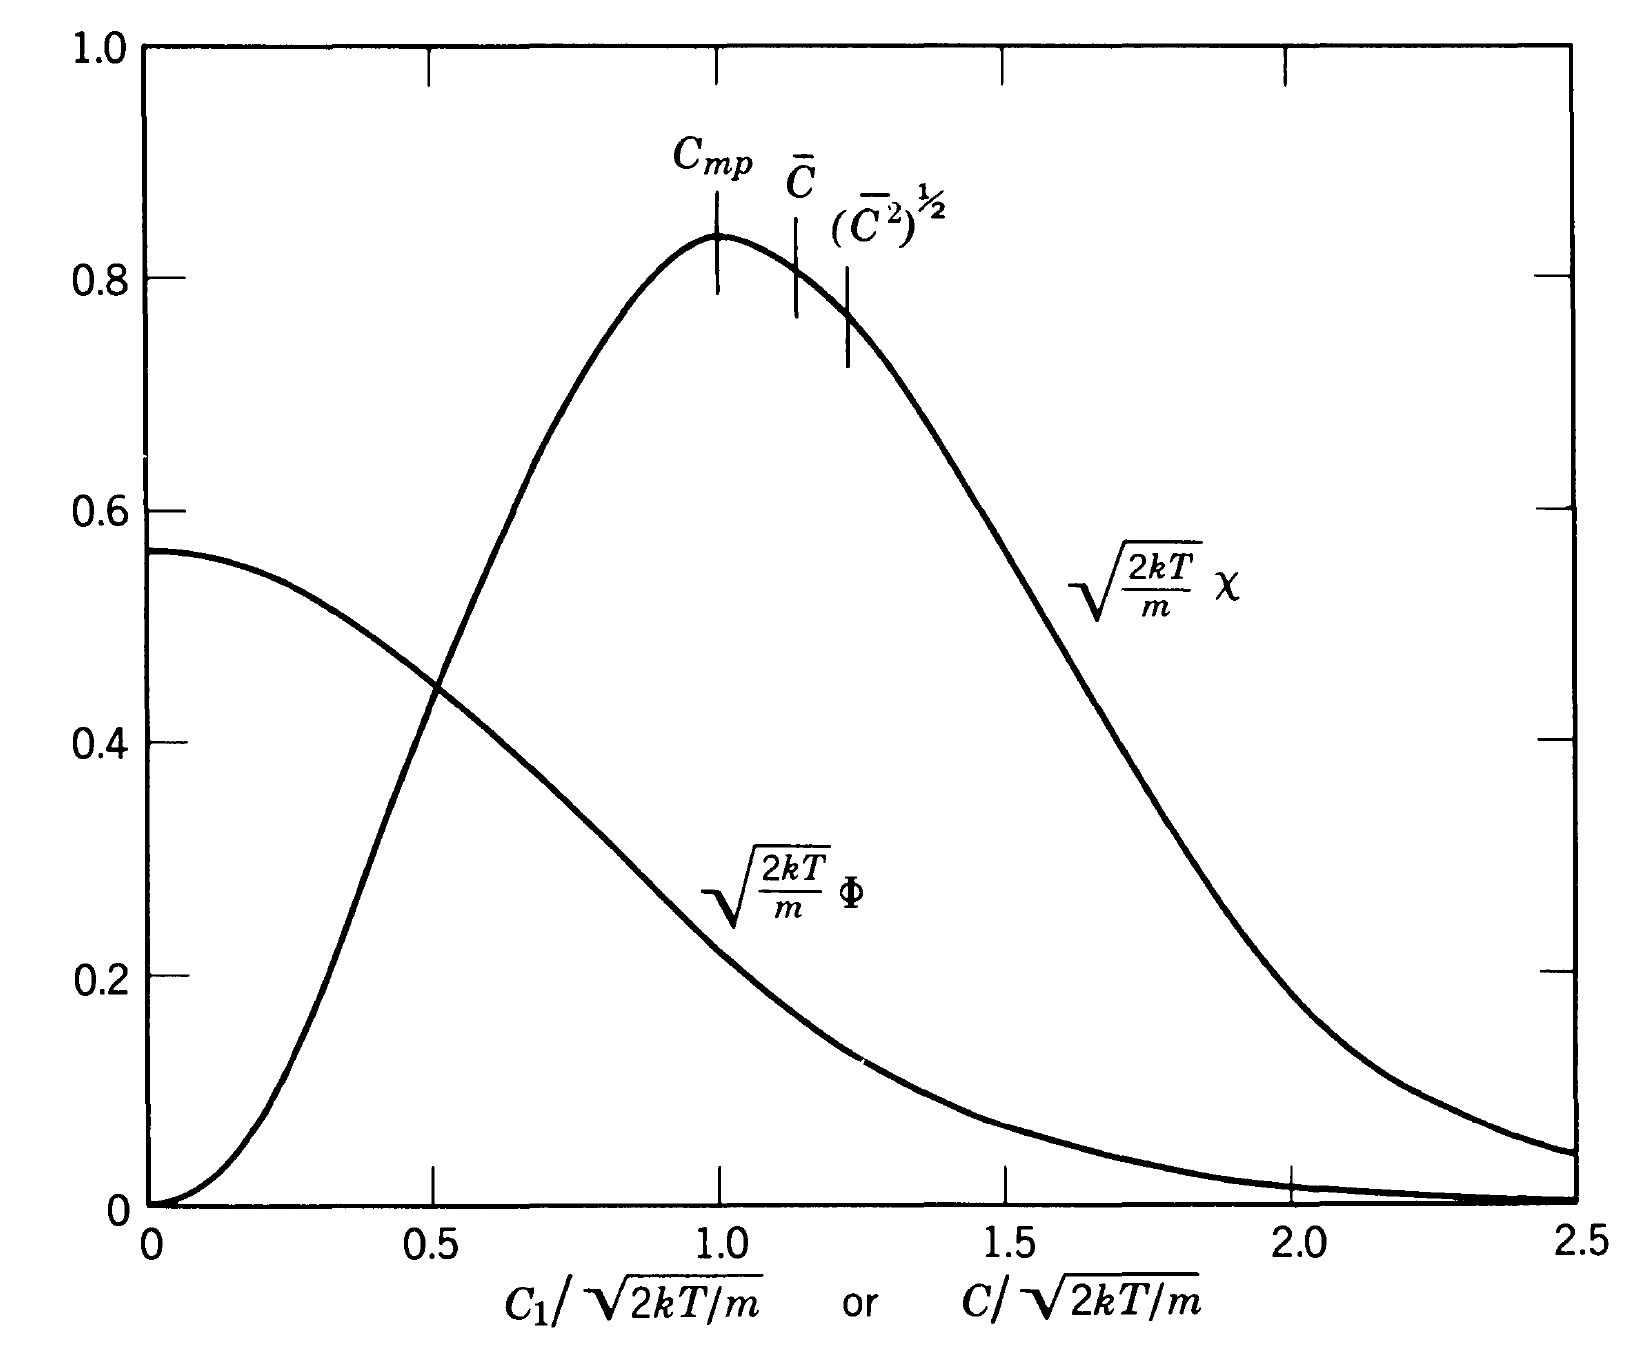
\includegraphics[width=0.55\textwidth]{Maxwellian.png}
        \caption{Distribution functions $\Phi$ and $\chi$.}
    \end{figure}
\end{frame}


\begin{frame}
\frametitle{Relative Velocity Distribution}
\begin{itemize}
    \item For a gas with two components \( A \) and \( B \), the relative velocity distribution function \( f(g_i) \) is also Maxwellian:
    \[
    f(g_i) = \left( \frac{m_{AB}^*}{2\pi k T} \right)^{3/2} \exp \left( - \frac{m_{AB}^* g_i^2}{2 k T} \right)
    \]
    \item Where \( m_{AB}^* \) is the reduced mass:
    \[
    m_{AB}^* = \frac{m_A m_B}{m_A + m_B}
    \]
\end{itemize}
\end{frame}

\begin{frame}
\frametitle{Relative Speed Distribution}
\begin{itemize}
    \item The relative speed distribution:
    \[
    \chi_M(g) dg = 4\pi g^2 \left( \frac{m_{AB}^*}{2 \pi k T} \right)^{3/2} \exp \left( - \frac{m_{AB}^* g^2}{2 k T} \right) dg
    \]
    \item This distribution is important for calculating collision frequencies between different species in a gas.
\end{itemize}
\end{frame}

% Slide 1: The Most Probable Speed
\begin{frame}{Most Probable Speed}
    The most probable speed \( C_{mp} \), as determined by the maximum of the Maxwell-Boltzmann distribution curve, is given by:
    \[
    C_{mp} = \left( \frac{2kT}{m} \right)^{1/2}
    \]
    This is the speed at which the largest number of gas molecules are moving.
\end{frame}

% Slide 2: Average Speed
\begin{frame}{Average Speed}
    The average speed \( \overline{C} \) is obtained by integrating over the velocity distribution function:
    \[
    \overline{C} = \int_0^{\infty} C \chi(C) dC
    \]
    Using known integrals, this evaluates to:
    \[
    \overline{C} = \frac{2}{\pi^{1/2}} \left( \frac{2kT}{m} \right)^{1/2} \approx 1.13 C_{mp}
    \]
    Thus, the average speed is slightly larger than the most probable speed.
\end{frame}

% Slide 3: Root-Mean-Square (RMS) Speed
\begin{frame}{Root-Mean-Square Speed}
    The root-mean-square speed \( \overline{C^2} \) is found by integrating over the square of the speed:
    \[
    \overline{C^2} = \int_0^{\infty} C^2 \chi(C) dC
    \]
    Which simplifies to:
    \[
    \overline{C^2}^{1/2} = \left( \frac{3kT}{m} \right)^{1/2} \approx 1.22 C_{mp}
    \]
    This gives the typical speed of a gas molecule considering the energy distribution.
\end{frame}

% Slide 4: Summary of Speeds
\begin{frame}{Summary of Speeds}
    The three characteristic speeds in the Maxwellian distribution:
    \begin{itemize}
        \item Most Probable Speed: \( C_{mp} \approx \left( \frac{2kT}{m} \right)^{1/2} \)
        \item Average Speed: \( \overline{C} \approx 1.13 C_{mp} \)
        \item RMS Speed: \( \overline{C^2}^{1/2} \approx 1.22 C_{mp} \)
    \end{itemize}
    
    These speeds are all of the same order of magnitude, increasing with temperature \( T \) and decreasing with molecular mass \( m \).
\end{frame}


\begin{frame}
\frametitle{Macroscopic Collision Rate}
We now use the Maxwellian velocity and speed distributions to develop
expressions for the collision rate and mean free path of a gas in thermal equilibrium.\\
\begin{itemize}
    \item For Maxwellian distributed velocities \( f_A(C_i) \) and \( f_B(Z_i) \), the macroscopic collision rate is:
    \[
    dZ_{AB} = n_A n_B g \sigma_T(g) f_M(C_i) f_M(Z_i) dV_C dV_Z
    \]
    \item This rate depends on the relative speed distribution and the total cross-section.
\end{itemize}
\end{frame}

\begin{frame}
\frametitle{Transform to Center of Mass Frame}
\begin{itemize}
    \item In the center of the mass frame, we transform the velocities:
    \[
    C_i = G_i - \frac{m_{AB}^*}{m_A} g_i, \quad Z_i = G_i + \frac{m_{AB}^*}{m_B} g_i
    \]
    \item Where \( G_i \) is the center of mass velocity and \( g_i = Z_i - C_i \) is the relative velocity.
    \item This simplifies the calculation of collision rates in many gas dynamics problems.
    \item Finally, after integrating over all $g_i$:

\[
dZ_{AB} = n_A n_B \left( \frac{m_{AB}^*}{2\pi k T} \right)^{3/2} e^{-\frac{m_{AB}^* g^2}{2 k T}} 4\pi g^2 \cdot g \sigma_T(g) dg
\]

\[
= n_A n_B \, g \, \sigma_T(g) \, \chi_M(g) dg.
\]

\end{itemize}
\end{frame}


\begin{frame}{Bimolecular Collision Rate}

By integrating over $g$  we obtain the final result called the bimolecular collision rate:
$$
Z_{\mathrm{AB}}=n_{\mathrm{A}} n_{\mathrm{B}} \sigma_{\mathrm{AB}} \sqrt{\frac{8 k T}{\pi m_{\mathrm{AB}}^*}}
$$

    For a hard-sphere collision between particles of two different species \( A \) and \( B \), the collision cross section is:
    \[
    \sigma_{AB} = \frac{\pi}{4} (d_A + d_B)^2
    \]
    More complex collision cross-sections depend on relative velocity and introduce a temperature dependence. \\
    \vspace{0.5cm}
    This cross-section appears in the rate of collisions between different species in a gas mixture.
\end{frame}

% Slide 2: Correction for Collision Counting
\begin{frame}{Correction for Collision Counting}
    In the analysis, we must correct for the fact that a collision between species \( A \) and species \( B \) is counted twice. This correction factor \( Z_{AB} \) is given by:
    \[
    Z_{AB} = \frac{1}{1 + \delta_{AB}} n_A n_B \sigma_{AB} \sqrt{\frac{8kT}{\pi m^*_{AB}}}
    \]
    Where \( \delta_{AB} \) is:
    \[
    \delta_{AB} = \begin{cases} 
        1, & \text{when } A = B \\
        0, & \text{when } A \neq B 
    \end{cases}
    \]
    This ensures proper counting of collisions in mixed gases. Each collision involving a species
A particle determines a free path length for species A collisions. When two species A particles collide, two free paths for species A are terminated simultaneously. We need to find the mean value of all free paths for species A.
\end{frame}

% Slide 1: Rate of Ending Free Paths
\begin{frame}{Rate of Ending Free Paths for Species A}
    The rate of ending free paths per particle of species \( A \) due to collisions with species \( B \) is:
    \[
    \Theta_A = \sum_{i=1}^{N_s} \Theta_{Ai} = \sqrt{\frac{8kT}{\pi}} \sum_{i=1}^{N_s} n_i \sigma_{Ai} \sqrt{\frac{1}{m_A} + \frac{1}{m_i}}
    \]
    This accounts for the contribution of all other species to the gas mixture.
\end{frame}

% Slide 2: Average Speed of Species A
\begin{frame}{Average Speed of Species A}
    The average speed of species \( A \) in the gas mixture is given by:
    \[
    \langle C_A \rangle = \sqrt{\frac{8kT}{\pi m_A}}
    \]
    This is the average distance traveled by a particle of species \( A \) per unit time.
\end{frame}

% Slide 3: Mean Free Path of Species A
\begin{frame}{Mean Free Path of Species A}
    The mean free path \( \lambda_A \) of species \( A \) in a gas mixture at equilibrium is:
    \[
    \lambda_A = \frac{\langle C_A \rangle}{\Theta_A} = \frac{1}{\sum_{i=1}^{N_s} n_i \sigma_{Ai} \sqrt{1 + \frac{m_A}{m_i}}}
    \]
    For a simple gas, where \( N_s = 1 \), this simplifies to:
    \[
    \lambda = \frac{1}{\sqrt{2} n \sigma}
    \]
    This represents a more accurate result compared to previous models.
\end{frame}


\begin{frame}
\frametitle{Molecular Magnitudes}

We are now in a position to use macroscopic measurements to estimate the magnitudes involved in molecular phenomena. Among the quantities that can be measured macroscopically are pressure $p$, density $\rho$, dynamic viscosity $\mu$, and molecular weight $M$, where $M$ is the molecular weight (mass per mole). We aim to find four quantities that characterize the molecular model: $m$, $d$, $n$, and $\sqrt{\overline{C^2}}$. Since $m = \frac{M}{N_A}$, determining $m$ also entails determining Avogadro's number $N_A$.
\end{frame}

\begin{frame}
\frametitle{Molecular Magnitudes}

We can use macroscopic measurements to estimate the magnitudes involved in molecular phenomena. Measurable quantities include:
\begin{itemize}
    \item Pressure $p$
    \item Density $\rho$
    \item Dynamic viscosity $\mu$
    \item Molecular weight $\hat{M}$ (mass per mole)
\end{itemize}

We aim to determine four key molecular model parameters:
\begin{itemize}
    \item Molecular mass $m$
    \item Molecular diameter $d$
    \item Number density $n$
    \item Root-mean-square molecular speed $\sqrt{\overline{C^2}}$
\end{itemize}

Since $m = \frac{\hat{M}}{N_A}$, where $N_A$ is Avogadro's number, determining $m$ also provides $N_A$.
\end{frame}

\begin{frame}
\frametitle{Macroscopic Properties of Air (SI Units)}

For air under standard conditions at $0^\circ$C and 1 atm, we have:
\begin{itemize}
    \item $p = 1.013 \times 10^5 \, \text{Pa}$ (pressure)
    \item $\rho = 1.288 \, \text{kg/m}^3$ (density)
    \item $\mu = 1.71 \times 10^{-5} \, \text{Pa s}$ (dynamic viscosity)
\end{itemize}

We assume air behaves as a single gas with molecular weight $\hat{M} \approx 28.9 \, \text{g/mol}$.
\end{frame}

\begin{frame}
\frametitle{Root-Mean-Square Molecular Speed}

The root-mean-square molecular speed $\sqrt{\overline{C^2}}$ is estimated using:
\[
\sqrt{\overline{C^2}} = \sqrt{\frac{3p}{\rho}} \approx 500 \, \text{m/s}
\]

This estimation provides the average velocity of air molecules under standard conditions.
\end{frame}

\begin{frame}
\frametitle{Estimating Molecular Diameter and Avogadro's Number}

We can estimate the molecular diameter $d$ and Avogadro's number $N_A$ from kinetic theory and viscosity. The dynamic viscosity relation is:
\[
\mu = \frac{1}{2} \rho \overline{C} \frac{m}{\sqrt{2\pi} d^2}
\]
Using:
\[
\overline{C} \approx \sqrt{\overline{C^2}} \quad \text{and} \quad N_A d^2 \approx \frac{\hat{M} \sqrt{\overline{C^2}}}{9 \mu}
\]
We find that:
\[
d \approx 3.7 \times 10^{-10} \, \text{m} \quad \text{and} \quad N_A \approx 6.7 \times 10^{23} \, \text{mol}^{-1}
\]
These values are consistent with empirical data for air.
\end{frame}


\begin{frame}
\frametitle{Molecular Mass and Number Density}

The accepted value of Avogadro's number from accurate measurements is:
\[
N_A = 6.02252 \times 10^{23} \, \text{mol}^{-1}
\]
From this, we can calculate the mass of a single molecule:
\[
m = \frac{\hat{M}}{N_A} \approx 4.80 \times 10^{-26} \, \text{kg}
\]
The number density of molecules $n_0$ at standard conditions (1 atm, 0$^\circ$C) is:
\[
n_0 = \frac{\rho}{m} \approx 2.69 \times 10^{25} \, \text{m}^{-3}
\]
This is the number of molecules per cubic meter of air. The same result can be obtained using the ideal gas equation $p = n k_B T$.
\end{frame}

\begin{frame}
\frametitle{Mean Spacing, Mean Free Path, and Collision Frequency}

The average molecular spacing $\delta$ is:
\[
\delta = \frac{1}{n_0^{1/3}} \approx 3.3 \times 10^{-8} \, \text{m}
\]
The mean free path $\lambda$ is:
\[
\lambda = \frac{1}{\sqrt{2} \pi n_0 d^2} \approx 6 \times 10^{-8} \, \text{m}
\]
The frequency of molecular collisions $\Theta$ is given by:
\[
\Theta = \frac{\overline{C}}{\lambda} \approx 10^{10} \, \text{sec}^{-1}
\]
\end{frame}

\begin{frame}
\frametitle{Comparison of Microscopic Distances}

We now compare the various molecular distances:
\[
\frac{\lambda}{\delta} : \frac{\delta}{d} \sim 170:10:1
\]
This shows that the mean free path is much greater than the average molecular spacing, which is much greater than the molecular diameter. The range of intermolecular forces is based on the order of the molecular diameter, which justifies the assumption that molecules interact only during short collisions.

This assumption remains valid if the gas density is not too high.
\end{frame}

\begin{frame}
\frametitle{The Scale of Molecular Distances}

The vastness of molecular distances and the high number density can be difficult to grasp. However, consider the following:\vskip0.5cm
\begin{quote}
\textit{
A man is known to breathe out about 400 c.c. of air at each breath, so a single breath of air must contain about $10^{22}$ molecules. The whole atmosphere of the earth consists of about $10^{44}$ molecules. Thus, one molecule bears the same relation to a breath of air as the latter to the whole atmosphere of the earth. If we assume that the last breath of, say, Julius Caesar has by now become thoroughly scattered through the atmosphere, then the chances are that each of us inhales one molecule of it with every breath we take. A man’s lungs hold about 2000 c.c. of air so the chances are that in the lungs of each of us, there are about five molecules from the last breath of Julius Caesar.
}
\end{quote}
\end{frame}


% Slide with questions 1-4
\begin{frame}
\frametitle{Practice Questions (1-4)}
\begin{enumerate}
    \item Describe the key differences between the classical thermodynamic approach and the kinetic theory approach to gas behavior.
    \item Explain the significance of the Maxwell-Boltzmann distribution in kinetic theory.
    \item How is the mean free path of gas molecules defined, and what factors influence its magnitude?
    \item What role do particle collisions play in the transport properties (viscosity, thermal conductivity, diffusion) of gases?
\end{enumerate}
\end{frame}

% Slide with questions 5-8
\begin{frame}
\frametitle{Practice Questions (5-8)}
\begin{enumerate}
    \setcounter{enumi}{4}
    \item Explain the concept of a velocity distribution function and how it is used to determine the macroscopic properties of a gas.
    \item Discuss how elastic collisions maintain equilibrium in a gas, and describe what happens to the velocity distribution in nonequilibrium conditions.
    \item What is the difference between the most probable speed, the average speed, and the root-mean-square speed in a Maxwellian distribution?
    \item Describe the assumptions made when deriving the perfect gas law from kinetic theory.
\end{enumerate}
\end{frame}

% Slide with questions 9-12
\begin{frame}
\frametitle{Practice Questions (9-12)}
\begin{enumerate}
    \setcounter{enumi}{8}
    \item In kinetic theory, what is the importance of the molecular cross-section, and how does it affect the collision frequency?
    \item Explain how the distribution function \( f(C_i) \) is used to calculate the number flux of molecules in a specific direction.
    \item What is the physical meaning of the relative velocity \( g_i \) between two colliding particles, and how is it related to the collision cross-section?
    \item Describe how the concept of detailed balance is applied to molecular collisions in a gas at equilibrium.
\end{enumerate}
\end{frame}

% Slide with questions 13-16
\begin{frame}
\frametitle{Practice Questions (13-16)}
\begin{enumerate}
    \setcounter{enumi}{12}
    \item What is the significance of the "differential cross-section" \( \left( \frac{d\sigma}{d\Omega} \right) \) in elastic collisions, and how is it used to compute the total cross-section?
    \item Explain how the Maxwellian velocity distribution leads to the ideal gas law \( pV = nRT \) in equilibrium.
    \item Define the term "mean collision frequency" and explain how it is calculated for a gas in thermal equilibrium.
    \item How does the variable hard sphere (VHS) model improve upon the simple hard sphere model in kinetic theory?
\end{enumerate}
\end{frame}

% Slide with questions 17-20
\begin{frame}
\frametitle{Practice Questions (17-20)}
\begin{enumerate}
    \setcounter{enumi}{16}
    \item Describe the relationship between the molecular diameter, number density, and collision frequency in determining the mean free path of gas molecules.
    \item What is the bimolecular collision rate, and how is it calculated for a gas mixture consisting of two species \( A \) and \( B \)?
    \item How is the Maxwellian speed distribution derived from the velocity distribution, and what does it represent?
    \item Discuss the physical significance of the root-mean-square molecular speed \( \overline{C^2}^{1/2} \) and how it relates to the thermal energy of the gas.
\end{enumerate}
\end{frame}

% Closing slide
\begin{frame}
    \frametitle{Good Luck!}
    These questions cover a broad range of theoretical concepts in kinetic theory. Review the underlying principles and practice deriving key equations to prepare for exams and practical applications.
\end{frame}

\end{document}



\end{document}




\end{document}
